\documentclass[20pt, a4paper]{report}   
%\documentclass[twocolumn]{report}   
\usepackage[utf8]{inputenc}
\usepackage[T1]{fontenc}
\usepackage{listings}

\usepackage[francais]{babel}
\usepackage{url} 
\usepackage{lmodern} 
\usepackage{geometry}  
\usepackage{graphicx}

%% Pour pouvoir mettre une image dans la page de garde
%% Le fichier .sty se trouve dans le dossier extensions-tex/
\usepackage{titlepic}

\usepackage{fancyhdr}
\usepackage[absolute]{textpos} 
\usepackage{wrapfig}
\usepackage{graphicx}
\usepackage{subfig}
\usepackage{float}
\usepackage{lscape}              % Pour pouvoir passer en paysage
\usepackage{multicol}            % Pour pouvoir faire plusieurs colonnes
\usepackage{makeidx}             % Pour crééer un index
\usepackage{setspace}            % Pour l'interligne de 1.5
\usepackage{endnotes}            % Pour les notes en fin de doc
\usepackage{footnote}            % Pour les notes en bas de page
\usepackage{soul}
\usepackage{amssymb}
\usepackage{multirow} 
\usepackage{colortbl}

% Pour avoir accès aux fonctions de conversions
% après import du package layouts on peut par exemple utiliser la commande 
% \printinunitsof{cm}\prntlen{\textwidth} qui affiche la largeur du texte en cm.
% exemple d'affichage : textwidth in cm : 15.99773 cm  

\usepackage{layouts}            

\makeindex
\usepackage{color}
\definecolor{gray}{rgb}{0.4,0.4,0.4}
\definecolor{darkblue}{rgb}{0.0,0.0,0.6}
\definecolor{cyan}{rgb}{0.0,0.6,0.6}


\lstset{
  basicstyle=\ttfamily,
  columns=fullflexible,
  showstringspaces=false,
  commentstyle=\color{gray}\upshape
}


%% le langage XML est peu supporté, donc je défini moi même les couleurs des
%% mots-clefs, en reprenant un post sur internet
\lstdefinelanguage{XML}{
  morestring=[b]",
  morestring=[s]{>}{<},
  morecomment=[s]{<?}{?>},
  stringstyle=\color{black},
  identifierstyle=\color{darkblue},
  keywordstyle=\color{cyan},
  morekeywords={xmlns,version,type},% list your attributes here
  % sets the caption-position to bottom
  captionpos=b
}

\definecolor{javared}{rgb}{0.6,0,0} % for strings
\definecolor{javagreen}{rgb}{0.25,0.5,0.35} % comments
\definecolor{javapurple}{rgb}{0.5,0,0.35} % keywords
\definecolor{javadocblue}{rgb}{0.25,0.35,0.75} % javadoc
	 
\lstset{language=Java,
basicstyle=\ttfamily,
keywordstyle=\color{javapurple}\bfseries,
stringstyle=\color{javared},
commentstyle=\color{javagreen},
morecomment=[s][\color{javadocblue}]{/**}{*/},
tabsize=4,
showspaces=false,
showstringspaces=false}

\definecolor{javared}{rgb}{0.6,0,0} % for strings
\definecolor{javagreen}{rgb}{0.25,0.5,0.35} % comments
\definecolor{javapurple}{rgb}{0.5,0,0.35} % keywords
\definecolor{javadocblue}{rgb}{0.25,0.35,0.75} % javadoc

\lstdefinelanguage{scala}{
  morekeywords={%
          abstract,case,catch,class,def,do,else,extends,%
          false,final,finally,for,forSome,if,implicit,import,lazy,%
          match,new,null,object,override,package,private,protected,%
          return,sealed,super,this,throw,trait,true,try,type,%
          val,var,while,with,yield},
  otherkeywords={=>,<-,<\%,<:,>:,\#,@},
  sensitive=true,
  keywordstyle=\color[rgb]{0,0,1},
  morecomment=[l]{//},
  morecomment=[n]{/*}{*/},
  basicstyle=\ttfamily,
  keywordstyle=\color{javapurple}\bfseries,
  stringstyle=\color{javared},
  commentstyle=\color{javagreen},
  morestring=[b]",
  morestring=[b]',
  morestring=[b]""",
  %% lstlisting ne gère pas les accents (c'est écrit dans la doc).
  %% Pour contourner ce problème, on peut énumérer les caractères qu'on va utiliser
  %% avec literate et extendedchars=true.
  %% Pour chaque accent il faut placer le caractère entre accolades (ex {à}) et
  %% ensuite écrire la traduction entre double accolades (ex {{à}}) et enfin écrire
  %% le nombre (1) . Entre deux entrées, on peut mettre des espaces pour plus de
  %% clareté.
  literate={é}{{\'e}}1 {è}{{\`e}}1 {à}{{\`a}}1 {ç}{{\c{c}}}1 {œ}{{\oe}}1 {ù}{{\`u}}1
  {É}{{\'E}}1 {È}{{\`E}}1 {À}{{\`A}}1 {Ç}{{\c{C}}}1 {Œ}{{\OE}}1 {Ê}{{\^E}}1
  {ê}{{\^e}}1 {î}{{\^i}}1 {ô}{{\^o}}1 {û}{{\^u}}1 {dollar}{{\$}}1
}[keywords,comments,strings]


\usepackage{textcomp}
\usepackage{listings}
\usepackage{color}

\definecolor{lightgray}{rgb}{.9, .9, .9}
\definecolor{darkgray}{rgb}{.4, .4, .4}
\definecolor{purple}{rgb}{0.65, 0.12, 0.82}

\lstdefinelanguage{JavaScript}{
  keywords={typeof, new, true, false, catch, function, return, null, catch, switch, var, if, in, while, do, else, case, break},
  keywordstyle=\color{blue}\bfseries,
  ndkeywords={class, export, boolean, throw, implements, import, this},
  ndkeywordstyle=\color{darkgray}\bfseries,
  identifierstyle=\color{black},
  sensitive=false,
  comment=[l]{//},
  morecomment=[s]{/*}{*/},
  commentstyle=\color{purple}\ttfamily,
  stringstyle=\color{red}\ttfamily,
  morestring=[b]',
  morestring=[b]",
  extendedchars=true,
  basicstyle=\footnotesize\ttfamily,
  showstringspaces=false,
  showspaces=false,
  frame=single,                   % adds a frame around the code
  %% numbers=left,
  numberstyle=\footnotesize,
  numbersep=9pt,
  tabsize=2,
  breaklines=true,
  showtabs=false,
  captionpos=b,
  %% lstlisting ne gère pas les accents (c'est écrit dans la doc).
  %% Pour contourner ce problème, on peut énumérer les caractères qu'on va utiliser
  %% avec literate et extendedchars=true.
  %% Pour chaque accent il faut placer le caractère entre accolades (ex {à}) et
  %% ensuite écrire la traduction entre double accolades (ex {{à}}) et enfin écrire
  %% le nombre (1) . Entre deux entrées, on peut mettre des espaces pour plus de
  %% clareté.
  extendedchars=true,
  literate={é}{{\'e}}1 {è}{{\`e}}1 {à}{{\`a}}1 {ç}{{\c{c}}}1 {œ}{{\oe}}1 {ù}{{\`u}}1
  {É}{{\'E}}1 {È}{{\`E}}1 {À}{{\`A}}1 {Ç}{{\c{C}}}1 {Œ}{{\OE}}1 {Ê}{{\^E}}1
  {ê}{{\^e}}1 {î}{{\^i}}1 {ô}{{\^o}}1 {û}{{\^u}}1 {dollar}{{\$}}1
}




% Pour les marges de la page
\geometry{a4paper, top=2.5cm, bottom=3.5cm, left=2.5cm, right=2.5cm, marginparwidth=1.2cm}

\parskip=5pt                   % distance entre § (paragraphe)
\sloppy                        % respecter toujours la marge de droite 

% Pour les pénalités :
\interfootnotelinepenalty=250  % note de bas de page
\widowpenalty=150              % veuves et orphelines
\clubpenalty=150 

% Pour la longueur de l'indentation des paragraphes
\setlength{\parindent}{15mm}


\usepackage[colorlinks=true,breaklinks=true]{hyperref}
\hypersetup{
  urlcolor=cyan           % color of external links
}

% j'indique à latex où aller chercher les images pour éviter d'avoir à taper le
% nom du dossier imgs/ à chaque fois que je veux inclure une image
\graphicspath{{imgs/}}



%%%%%%%%%%%%%%%%%%%%%%%%% MACRO %%%%%%%%%%%%%%%%%%%%%%%%%%%%%%%%%%%%%%%%%%%%%%%%
% macro pour enlever le nom 'chapitre'
\makeatletter
\def\@makechapterhead#1{%
  \vspace*{20\p@}%
          {\parindent \z@ \raggedright \normalfont
            \interlinepenalty\@M
            \ifnum \c@secnumdepth >\m@ne
            \Huge\bfseries \thechapter\quad
            \fi
            \Huge \bfseries #1\par\nobreak
            \vskip 20\p@
          }
}

\def\@makeschapterhead#1{%
  \vspace*{20\p@}%
          {\parindent \z@ \raggedright
            \normalfont
            \interlinepenalty\@M
            \Huge \bfseries  #1\par\nobreak
            \vskip 20\p@
          }
}
\makeatother

% definir l'apparence des numeros des endnotes :
\renewcommand{\enoteformat}{
  \rightskip 
  \leftskip
  \leavevmode
  \llap{\theenmark . }
}

%Pour avoir a la fois les footnotes et endnotes :
\newcommand{\mafootnote}[2]{
  \footnote{#2 \label{#1}}
  \stepcounter{endnote}
  \endnotetext{#2 (Note \ref{#1}, page \pageref{#1})}
}

%%%%%%%%%%%%%%%%%%%%%% PAGE DE GARDE %%%%%%%%%%%%%%%%%%%%%%%%%%%%%%%%%%%%%%%%%%%
% Page de garde personnalisée Début

\titlepic{
  
\includegraphics[width=.4\linewidth]{imgs/universite-marne-la-vallee.jpg}
  
\includegraphics[width=.4\linewidth]{imgs/mimesis.png}
}

\title
    {   \vspace{-55mm}
      \normalsize{Université Paris-Est Marne-la-Vallée\\
        2011-2012}\\
      \vspace{70mm} 
      \Huge{\textbf{Rapport de stage en entreprise}}\\
      \huge{Interface Web pour piloter l'outil de déploiement du jeu en ligne
        sur le Cloud}\\
    }
    \author{\textbf{Vincent Munier} : \textit{vmunier@etudiant.univ-mlv.fr} \\
      M2 informatique : parcours logiciel\\
      \vspace{25mm} \\
      \today
    }
    \date{
      \normalsize{
        \vspace{40mm}
        Maître de stage : Damian Arregui\\
        Responsable de formation : Serge Midonnet\\
      }
    }


    %%%%%%%%%%%%%%%% RAPPORT %%%%%%%%%%%%%%%%%%%%%%%%%%%%%%%%%%%%%%%%%%%%%%%%%%%%%%%
    \begin{document}

    \maketitle

    \renewcommand{\abstractname}{Sujet de stage}
    \abstract{Le candidat rejoindra \textbf{l’équipe Infrastructure},
      responsable du cœur de l'architecture client/serveur de notre plateforme,
      ainsi que de son déploiement sur le Cloud. 

      Votre mission principale sera de développer une Interface Web 2.0 pour
      piloter notre outil de déploiement de jeu en ligne sur le Cloud. Cette
      interface est destinée à l'ensemble des équipes de production et
      d'opérations.

      Les technologies utilisées sont les suivantes : Java, Scala, Play
      Framework, JavaScript, HTML/CSS, ExtJS, Amazon Web Services, Chef, Ubuntu
      Linux.
    }

    \clearpage
    \tableofcontents
    \clearpage

    \begin{onehalfspace}           % Pour avoir un interligne de 1,5

      \chapter{Présentation de l'entreprise}

\section{L'entreprise : Mimesis Republic}

Co-fondée par Nicolas Gaume et Sébastian Lombardo en 2007, Mimesis Republic est
une société française basée à Paris et Bordeaux, spécialisée dans les
technologies plurimedia (réseaux sociaux, web, jeux vidéo). Composée d’une
équipe de 47 personnes et d’un management expérimenté, à l’origine de nombreux
blockbusters dans le secteur de l’entertainment depuis plus de 15 ans, Mimesis
Republic a placé le projet Mamba Nation au cœur de sa stratégie à destination
des adolescents et des jeunes adultes. Mimesis Republic est financée par des
investisseurs privés issus du monde de l’entreprise.

\section{Le projet : Mamba Nation}

Mamba Nation est un univers dédié aux adolescents et jeunes adultes qui
ambitionne de relier la vie réelle et le monde virtuel avec les réseaux sociaux
comme passerelle.

Cet univers virtuel est accessible au sein d'un navigateur internet à travers
une applet Java. L'intégralité de son contenu est \textit{streamé}, aucun client n'est à
installer sur l'ordinateur de l'utilisateur.

Mamba Nation c’est le renouveau du réseau social qui se construit sur Facebook
en y amenant l’Avatar, les jeux, les outils, les marques dont les ados et les
jeunes adultes ont besoin.
La véritable innovation pour les jeunes comme pour les marques, ce n’est pas de
choisir entre le réel et le virtuel, c’est d’utiliser le virtuel pour positiver
et enrichir sa vie réelle. C’est ce que nous appelons l’EXTRA LIFE.

Dans Mamba Nation, Vous pouvez vous faire des amis, vous amuser ensemble, et
même obtenir de la reconnaissance à travers une multitude d’actions et
d’interactions. En résumé «  FRIENDS + FUN + FAME ».

Ici le jeu n’est pas une fin, c’est un moyen permettant à chacun de s’engager et
révéler sa véritable personnalité, son véritable caractère.
Chaque utilisateur peut donc créer son Avatar, voir ses différents avatars,
chatter, inviter des amis, draguer, danser et chanter, etc…

Mamba Nation est génératrice de moments forts (virtuels) et partagés
(réellement).

\subsection{Images de l'univers virtuel} 

\begin{figure}[H]
  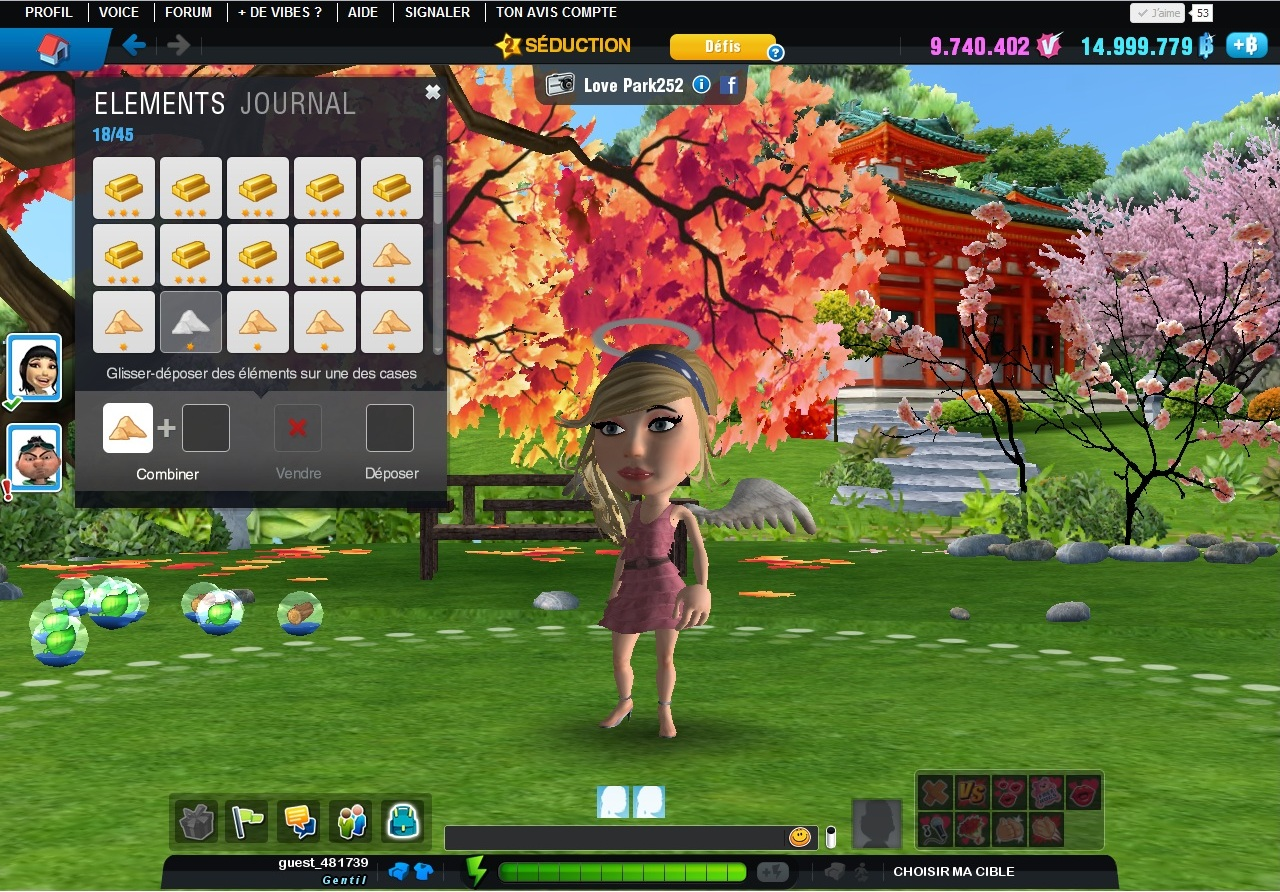
\includegraphics[width=\textwidth]{univers-gui-1.jpg}
  \caption{La GUI - 1}
\end{figure}


\begin{figure}[H]
    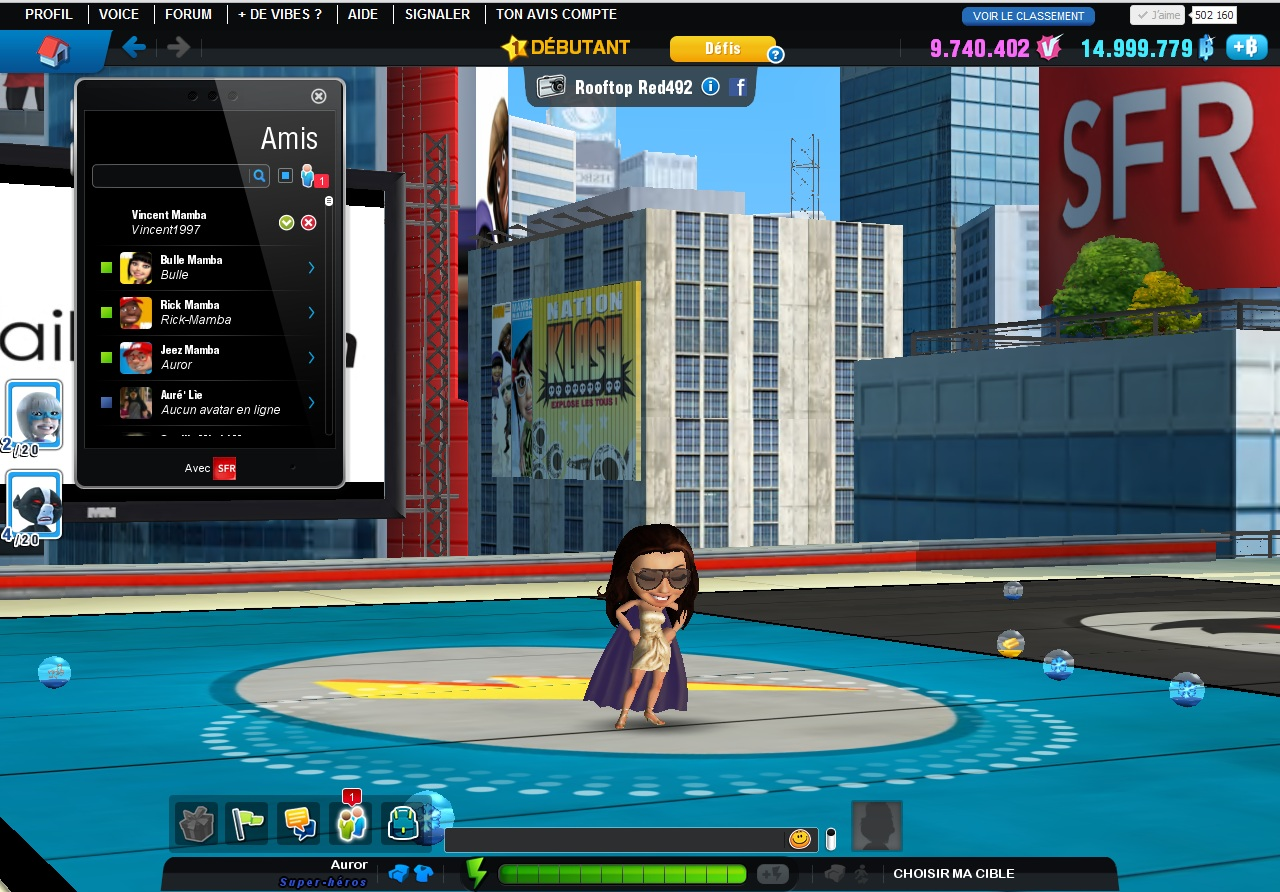
\includegraphics[width=\textwidth]{univers-gui-2.jpg}
  \caption{La GUI - 2}
\end{figure}


\begin{figure}[H]
  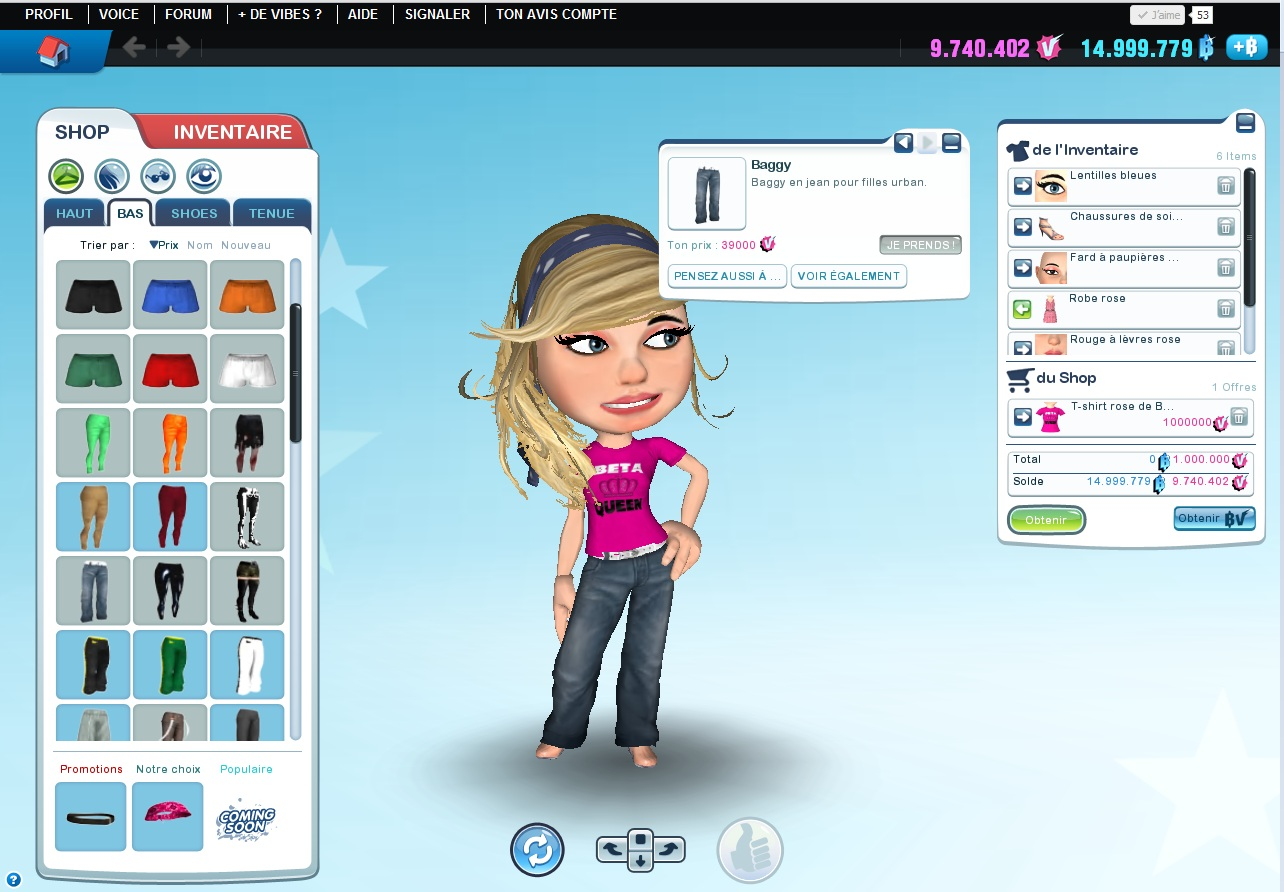
\includegraphics[width=\textwidth]{univers-shop.jpg}
  \caption{Le Shop}
\end{figure}

\begin{figure}[H]
  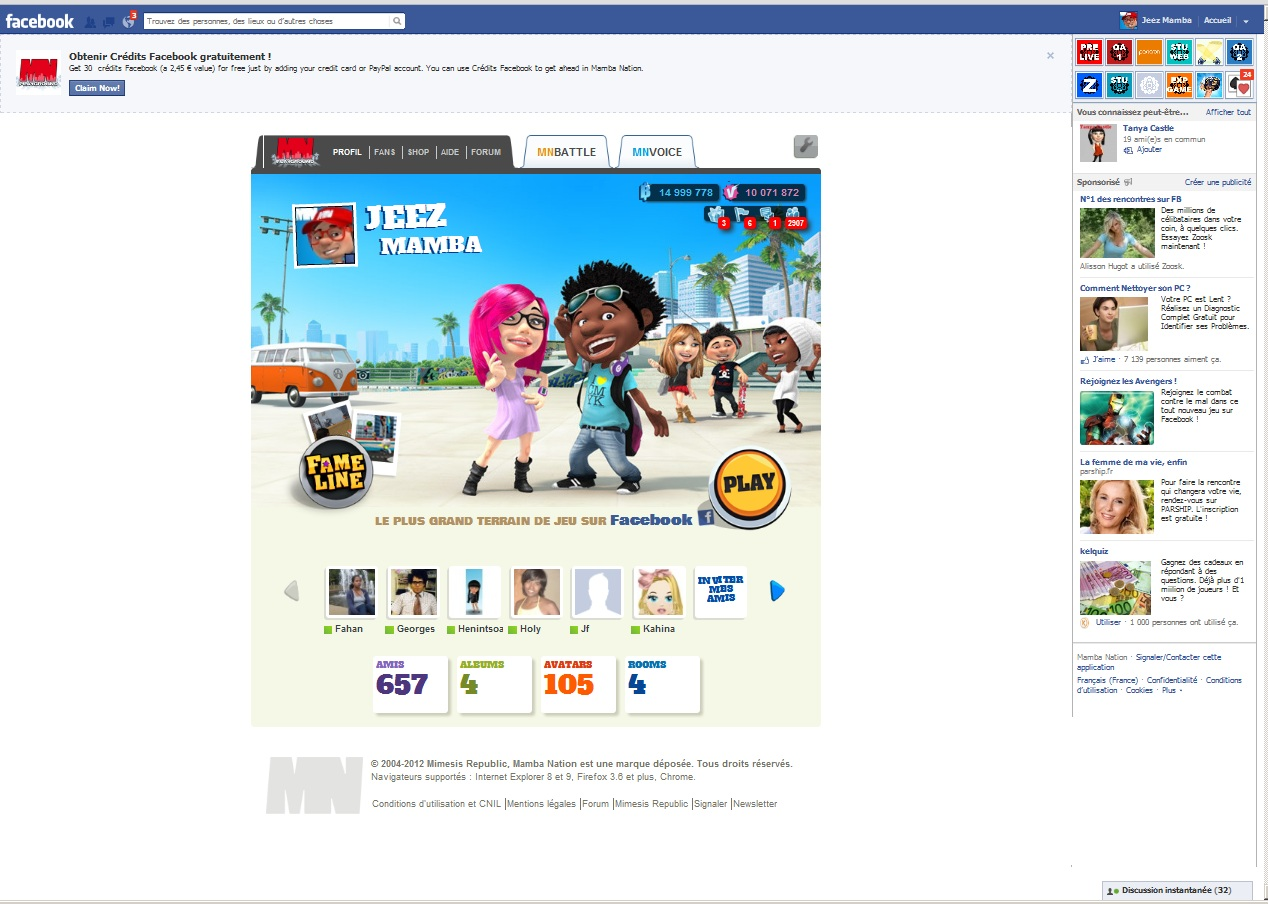
\includegraphics[width=\textwidth]{facebook.jpg}
  \caption{Facebook et Mamba Nation}
\end{figure}

\begin{figure}[H]
  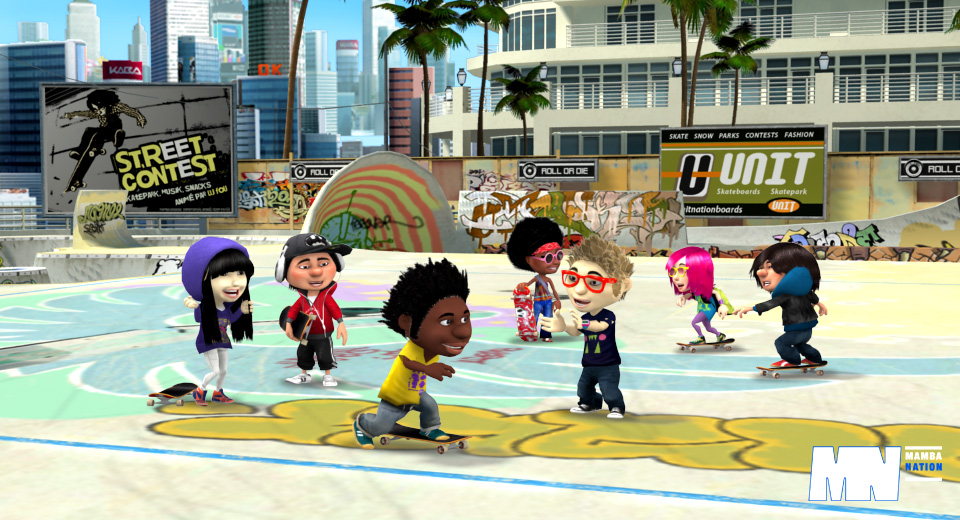
\includegraphics[width=\textwidth]{univers-skate.jpg}
  \caption{Tchater dans la Nation}
\end{figure}

\begin{figure}[H]
  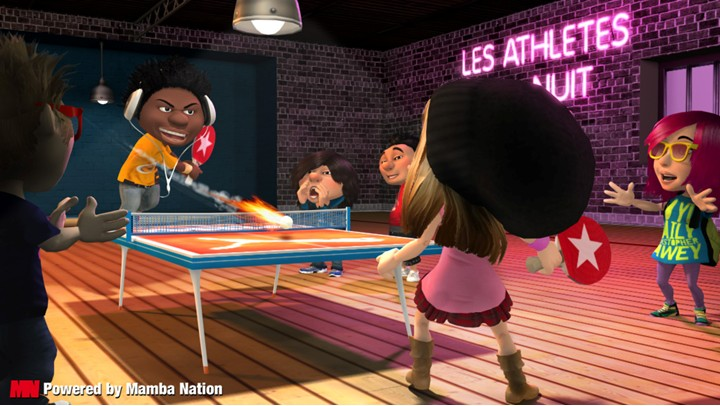
\includegraphics[width=\textwidth]{ping-pong.jpg}
  \caption{Une partie de ping pong dans la Nation}
\end{figure}

\begin{figure}[H]
  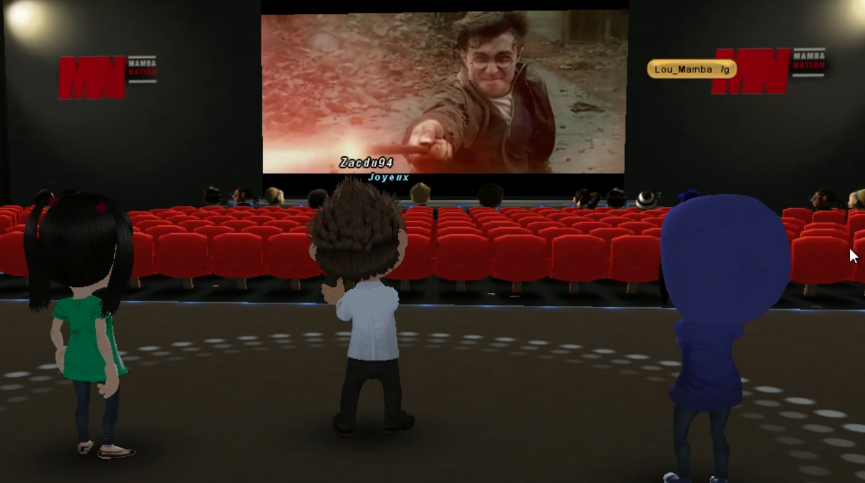
\includegraphics[width=\textwidth]{cinema.png}
  \caption{Regarder une vidéo Dailymotion en compagnie de ses potes}
\end{figure}


\section{Modèle économique}

La société mise sur un modèle Freemium, l'accès au service est gratuit, mais
pour obtenir ou utiliser certains biens virtuels tel que des vêtements ou des
animations d'avatar, les utilisateurs doivent acheter des "Blings" ou des
"Vibes", les monnaies virtuelles du site. La société vise un taux de 3 à 10\%
d'utilisateurs payant pour financer son service et être rentable sous 2 ans.

La société mise également sur la publicité et les évenements qu'elle organisera
dans ses salons 3D grâce à ces nombreux partenaires. Elle parle notamment de
concerts privées d'artiste avec leur avatar.

\section{Partenaires}

Mimesis Republic s'est entouré de partenaires importants pour développer son
produit notamment Xavier Niel, fondateur et vice-président du groupe Iliad, via
son fonds d’investissement Kima Ventures, Marc Simoncini, P-DG et fondateur du
site de rencontres Meetic, via son fonds d'investissement Jaina Capital, Steve
et Jean-Émile Rosenblum, fondateurs et dirigeants de Pixmania via leur fonds
d'investissement Dotcorp Asset Management, François Pinault, via sa holding
Artemis S.A, Laurent Schwarz co-fondateur d'Alten, Jean-François Cécillon ancien
président d'EMI France, Pascal Nègre P-DG de Universal Music France.

La société a annoncé qu'elle avait signé des partenariats pour enrichir son
univers virtuel avec :
\begin{itemize}
\item[\textbullet]\textbf{Universal Music} pour promouvoir et lancer des artistes,
  réaliser des évènement musicaux, etc.
\item[\textbullet]\textbf{Allociné} qui va animer des salons communautaires en
  3D autour de séries TV et de films
\item[\textbullet]\textbf{Puma} qui va associer la Mamba Nation à ses
  campagnes publicitaires, et apporter des items virtuels
\item[\textbullet]\textbf{Trace} qui va relooker l'habillage de ses chaînes de
  télévision (Trace TV, etc.) et de sa filiale de téléphonie mobile Trace
  Mobile
\item[\textbullet]\textbf{DailyMotion} qui va streamer de la vidéo au sein de
  l’expérience
\end{itemize}


\section{Les équipes}

\subsubsection{L'équipe Architecture}


\subsection{L'équipe Engine}
L'équipe Engine développe le moteur 3D de l'univers virtuel.
C'est aussi cette équipe qui développe les outils graphiques et les compilateurs
de contenus (Mesh, Animations,...).

 %% outils de productions d’assets 3DS Max (Editeur + Export)
 %% outils d’intégration des assets 3D (Builder)
 %% outils de visualisation et de tests des assets dans le moteur 3D (Runtime)
 %% fonctionnalités dans le moteur 3D sur demandes des équipes graphiques

\subsection{L'équipe Infrastructure}
L'équipe Infrastructure est responsable du cœur de l'architecture client/serveur
de la plateforme, ainsi que de son déploiement sur le Cloud.
J'ai rejoint cette équipe pour mon stage.

\subsection{L'équipe Studio}

L'équipe studio se concentre sur les minijeux facebook. Ces minijeux ont pour
but final d'attirer les joueurs dans l'univers 3D Mamba Nation.

\subsection{L'équipe Expérience}

L'équipe expérience travaille sur le Gameplay du jeu. Les développeurs de cette
équipe implémentent toutes les mécaniques et règles du jeu dans la Nation.

\begin{figure}[H]
  \begin{center}
    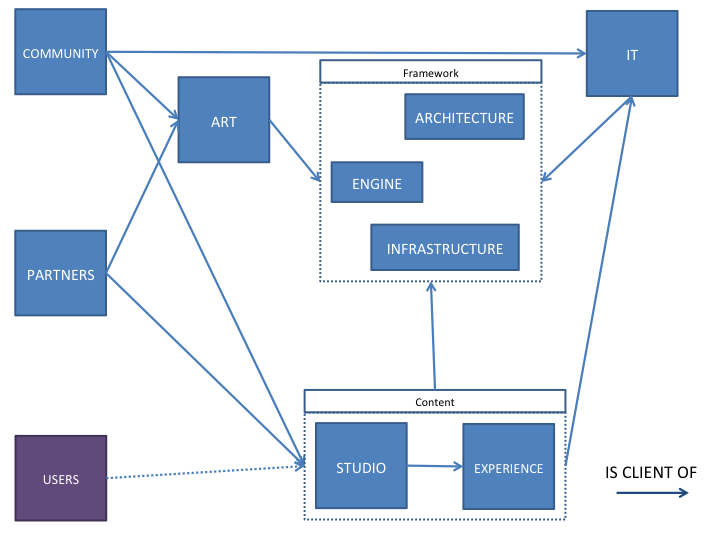
\includegraphics[width=\textwidth]{organisation.png}   
  \end{center}
  \caption{Les relations client/fournisseur}
\end{figure}


      \chapter{Les outils}       
Les outils occupent une part importante du stage.
L'équipe de Mimesis Republic est à la pointe de la technologie et utilise de
nombreux outils pour accélérer le développement.\\
La plupart de ces outils sont open source, un certain nombre sont assez jeunes
et rarement utilisés par les entreprises en général, qui ne prennent
probablement pas le risque de s'engager avec des nouveaux outils.\\ 
Ceux-ci demandent effectivement un effort d'apprentissage et d'adaptation au
début mais une fois maîtrisés, le gain de productivité est réel.\\

%% Le panel de technologies utilisées 
%% Scala, Play!, jQuery, CoffeeScript, SBT, Mercurial, AWS, Chef.

Je décris ci dessous chacun de ces outils,
classés par temps d'utilisation dans le travail que j'ai effectué.
Les outils que j'ai le plus utilisés sont présentés en premier et sont décrits
de façon plus complète, avec leurs avantages et inconvénients.

\section{Scala}
Scala est le langage de programmation utilisé pour développer l'univers \textit{Mamba
  Nation}.\\
Le moteur 3D du jeu est codé en Scala, les mécaniques de gameplay sont codés en
Scala, l'outil d'infrastructure coté serveur est aussi codé en Scala.

C'est un langage de programmation multi-paradigme conçu à l'École polytechnique
fédérale de Lausanne (EPFL).
Son nom vient de l'anglais Scalable language qui signifie  ``langage évolutif''
. 

\subsection{Caractéristiques et points forts de Scala}

\begin{itemize}
\item[\textbullet]\textbf{Tourne sur la JVM :}\\
  Il est prévu pour être compilé en bytecode Java (exécutable sur la JVM).
  Il existe aussi un portage sur la machine virtuel .Net qui reste néanmoins
  moins abouti que pour la JVM.\\

  Si on souhaite utiliser Scala exclusivement avec la JVM, il est alors possible
  d'utiliser les bibliothèques écrites en Java de façon complètement
  transparente. Ainsi, Scala bénéficie de la maturité et de la diversité des
  bibliothèques qui ont fait la force de Java depuis une dizaine d'années.\\

\item[\textbullet]\textbf{Tout dans les bibliothèques :}\\
  Le coeur du langage est minimal, la plupart des fonctionnalités majeures se
  trouvent être implémentées dans des bibliothèques.\\
  C'est un point important pour l'évolutivité du langage.\\

  Un exemple : les collections standards scala sont faciles à utiliser, concises
  et semblent faire partie du langage même si elles sont en fait implémentées
  dans une bibliothèque.\\
  Quelques lignes suffisent pour partitionner une liste \textit{people} en deux
  autres (\textit{minors} et \textit{adults}), en fonction de leur age :
\begin{verbatim}
    class Person(val name:String, val age:Int)
    val people = List(
    new Person("Hervé", 22),
    new Person("Julie", 17),
    new Person("Greg", 18))

    val (minors, adults) = people partition (_.age < 18)
\end{verbatim}
Ce morceau de code demanderait plusieurs boucles imbriquées en Java.\\
Ici, List est juste une classe et partition une méthode.\\
Ces fonctionnalités étant toutes implémentées dans des bibliothèques,
le programmeur peut lui aussi écrire ses propres bibliothèques qui seront
faciles d'utilisation, concises et extensibles.\\

\item[\textbullet]\textbf{Orienté objet pur :}
  \begin{itemize}
  \item Toute valeur est un objet \\
    1.hashCode renvoie 1
  \item Toute opération est un appel de méthode :\\
    le compilateur remplace 1 + 2 par (1) .+ (2)\\
  \end{itemize}
  Les exceptions à ces règles de Java ont été supprimées :\\
  Plus de primitives comme int, float (Int et Float à la place).\\
  Plus de qualificateur ``static'' mais un mot clef ``object'' qui équivaut à créer
  automatiquement un singleton thread safe en scala. \\
  Ces quelques changements contribuent à rendre le langage plus extensible
  que Java.\\
\item[\textbullet]\textbf{Fonctionnel :}\\ 
  Toutes les fonctions sont des valeurs et puisque toute valeur est objet en
  Scala, toute fonction est aussi un objet. 
  Scala offre une syntaxe légère pour les fonctions anonymes, supporte les
  fonctions de premier ordre, possède les case classes et le pattern matching.\\
  Par contre la récursion terminale n'est pas complètement supportée à cause du
  manque de support de la JVM pour la récursion terminale. Le compilateur Scala
  optimise les cas simples d'appels terminaux en boucle while.\\
\item[\textbullet]\textbf{Statiquement typé :}\\
  Scala est un langage fortement typé qui permet d'assurer une certaine sécurité
  dans les programmes, offrir de bonnes performances (aujourd'hui les langages
  statiquement typés ont tendance à être plus rapides que les langages
  dynamiquement typés) et facilite le refactoring de code car de nombreuses
  erreurs sont signalées par le compilateur lorsque un changement est effectué.\\

  Les types ne doivent pas être nécessairement indiqués car ils peuvent être
  inférés automatiquement par le compilateur dans la majorité des cas.\\
  L'indication des types reste obligatoire pour les paramètres de méthodes.\\
\item[\textbullet]\textbf{Autorise la Surcharge d'opérateurs :}\\
  Tout opérateur est une fonction. Une surcharge d'opérateur n'est rien d'autre
  qu'une surcharge de méthode en Scala.\\
\item[\textbullet]\textbf{Possède un interpréteur en ligne de commande :}\\ 
  Comme python et son ipython, Scala possède un environnement de programmation
  interactif en ligne de commande (REPL, read-eval-print-loop).\\
  Le REPL facilite grandement l'apprentissage d'un nouveau langage puisqu'il
  donne de rapides retours sur le code entré.\\
\item[\textbullet]\textbf{Trait :}\\Entre les interfaces Java et l'héritage
  multiple C++, les traits peuvent avoir des implémentations de méthode et des
  champs tout en rendant impossible l'héritage en diamant.\\
  Ruby est un autre langage qui possède les traits.\\  
\item[\textbullet]\textbf{Performant :}\\Les performances de Scala sont comparables
  à celles de Java. Le paradigme fonctionnel de Scala incite à utiliser des
  données immuables et favorise l'activation de certaines optimisations de la
  JVM.\\
  Papier publié par Google qui compare les performances de Java, C++, Go et Scala :
  \url{https://days2011.scala-lang.org/sites/days2011/files/ws3-1-Hundt.pdf}\\
\end{itemize}


La principale caractéristique qui rend le langage évolutif reste que Scala
fusionne les paradigmes fonctionnel et orienté objet à merveille, bien plus loin
que n'importe quel autre langage.\\
Je pense en particulier aux programmeurs OCaml qui peuvent, à souhait, utiliser
la programmation fonctionnel ou objet mais qui dans 90\% des cas d'utilisations
utilisent le coté fonctionnel du langage.\\
En Scala, la mixité entre les deux paradigmes est réelle avec une utilisation
légèrement supérieure de l'orienté objet (estimation grossière : 60\% objet, 40\%
fonctionnel).\\

Les paradigmes fonctionnel et orienté objet sont fondamentalement différents
et chacun possède des caractéristiques qui facilitent la résolution d'un type
de problème.\\
La complémentarité des paradigmes fonctionnel et orienté objet :\\\\
\begin{tabular}{|c|c|}
  \hline
  \textbf{fonctionnel} & \textbf{orienté objet}\\
  \hline
  Facilite la production de code simple & Facilite l'adaptation et l'extensibilité\\
  grâce aux fonctions de premier ordre, & de projets complexes grâce aux\\
  closures, et pattern matching & classes, sous typage et héritage \\
  \hline
\end{tabular}


\subsection{Faiblesses du langage}
\begin{itemize}
\item[\textbullet] Bien que le langage soit aujourd'hui mature et prêt à être utilisé en
  entreprise, peu ont fait le pas.\\
  Toutefois, quelques entreprises bien connus utilisent aujourd'hui Scala.
  C'est le cas de Twitter, LinkedIn et Foursquare qui ont incorporés Scala au
  coeur de leurs projets.\\
  Par exemple Twitter a transféré tout leur code coté serveur de Ruby en Scala,
  afin d'avoir les meilleurs performances possibles tout en gardant un langage
  extensible pouvant faire face à l'évolution croissante de leurs demandes.\\

  %% Parmi les sociétés qui utilisent Scala, nous pouvons citer :\\
  %% EDFT, Novell, the Guardian, Xebia, Xerox, Sony, Siemens, Thatcham,
  %% OPower, GridGain, AppJet, Reaktor, LinkedIn.\\

  Néanmoins, Scala reste pour l'instant un langage de niche avec une estimation
  de 0.237\% d'utilisation pour le mois de juillet 2012 calculée par le site
  \href{http://www.tiobe.com/index.php/content/paperinfo/tpci/index.html}{tiobe.com}.\\
\item[\textbullet] Les plugins IDE Scala progressent lentement et restent
  faibles en fonctionnalités comparés à ce qu'offrent les IDE Java.\\
\item[\textbullet] Le compilateur du langage, scalac, est lent
  (approximativement 10 fois plus lent que javac pour un nombre de lignes de
  code équivalent)\\
\end{itemize}

Pour finir cette présentation du langage, voici deux citations de deux
créateurs de langages :\\
\textbf{James Gosling}, créateur de Java :\\
``If I were to pick a language to use today other than Java, it would be
Scala.''\\\\
\textbf{James Strachan}, créateur de Groovy :\\
``I can honestly say if someone had shown me the Programming in Scala
book by Martin Odersky, Lex Spoon and Bill Venners back in 2003 I’d probably
have never created Groovy.''\\


%% ne pas utiliser l'indentation automatique sinon ça va décaler le code sur la
%% droite et ça ne tiendra pas sur le pdf
\clearpage
Équivalences de code Java, Scala :\\
\noindent
\small\addtolength{\tabcolsep}{-5pt}
\begin{tabular}{|c|c|}
  \hline
  \textbf{Java} & \textbf{Scala}\\
  \hline
  \lstset{language=Java}
  \begin{lstlisting}
boolean hasUpperCase = false
for (int i = 0; i < name.length(); i++)
  if (Character.isUpperCase(name.charAt(i))) {
    hasUpperCase = true;
    break;
  }
\end{lstlisting} &   \lstset{language=Scala}
\begin{lstlisting}
// Utilisation des collections et closures Scala
val hasUpperCase = name.exists(_.isUpper)
\end{lstlisting}
\\
\hline
\lstset{language=Java}
\begin{lstlisting}
public class Person {
  private String name;
  private int age;
  public Person(String name, int age) {
    this.name = name; this.age = age;
  }

  public String getName() { return name;}
  public int getAge() { return age; }

  public void setName(String name) { 
    this.name = name; 
  }
  public void setAge(int age) { 
     this.age = age; 
  }
}
\end{lstlisting} &
\lstset{language=Scala}
\begin{lstlisting}
// Scala créé automatiquement les getters et
// setters pour 'name' et 'age'
class Person(var name: String, var age: Int)
\end{lstlisting}
\\
\hline
\end{tabular}


\section{Play!}

Play! est un framework MVC inspiré de Rails qui permet de créer facilement des
applications web avec Java et Scala.

\subsection{Full stack}
Play! embarque un serveur web, il se suffit à lui-même. Cette notion
est appelée “full-stack”. Elle signifie que Play! est autonome 
dans son mode de développement en proposant tout ce qu’il faut pour faire
une application web, de la couche présentation à l’accès aux données.
En production, les applications Play! s'exécutent grâce au serveur web intégré.

\subsection{Choix libre de la technologie coté client}

Le framework Play! ne s'occuppe que de la partie coté serveur.
Coté client, nous avons le choix des technologies (HTML5 + CSS3 + jQuery
par exemple).

Play! offre un support natif pour deux technologies clientes :
CoffeeScript et LESS.
\begin{itemize}
\item CoffeeScript est un petit langage qui compile vers du JavaScript.
  Il propose une syntaxe concise et permet d'éviter les nombreux pièges de
  JavaScript. Il y a une relation 1-1 entre du code JavaScript et du code
  CoffeeScript.
\item LESS est un petit langage lui aussi mais qui compile vers du CSS.
  Grace à LESS, il est possible de rajouter des variables, des opérations
  (comme additionner des couleurs ensemble) et faire de l'héritage dans nos
  fichiers de styles.
\end{itemize}

\bigskip

CoffeeScript a été utilisé pour le développement du projet mais le besoin
d'utiliser LESS ne s'est pas fait sentir.

\subsection{Architecture stateless}

Play! est stateless, le serveur n'a aucune vision du client.
Il n'existe pas d'état (session) côté serveur, l'état est stocké coté client (dans
des cookies et cache) et/ou en BDD.
\bigskip

C'est la requête qui ``porte'' toutes les informations nécessaires à l'exécution
de l'action :\\
http://monsite/donne/moi/utilisateur/12 \\
Le serveur reçoit une requête, traite la requête puis renvoie une réponse.
Après envoie de la réponse, le client est oublié.

Dans une architecture stateful, l'historique d'activité du client sur le site
web va être gardé coté serveur (il est allé sur tel page, puis il a cliqué tel
bouton) alors que dans une architecture stateless, cette information n'est pas
gardé.

Une architecture stateless permet d'avoir de meilleurs performances et une
faible consommation mémoire. Play! offre de bonne performance car les requêtes
peuvent être traîtées : 
\begin{itemize}
\item dans le désordre
\item par 2 (ou+) serveurs différents
\end{itemize}
et Play! consomme peu de mémoire car :
\begin{itemize}
\item il n'y a pas de session sauvegardée coté serveur
\item il n'y a pas de réplication de session
\end{itemize}

\subsection{Rechargement à chaud et affichage des erreurs dans le navigateur}

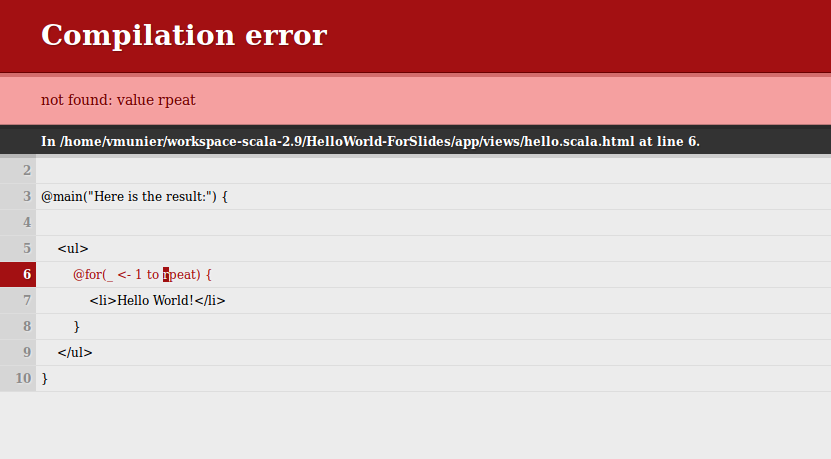
\includegraphics[scale=0.40]{play-erreur.png}  

Le cycle de développement est rapide, edition $\rightarrow$ test $\rightarrow$ correction.
Avec Play! il y a un seul endroit où consulter le résultat de son
application : le navigateur. 

Avec des frameworks web Java classiques (JSF par exemple), une erreur peut se
produire à plein d'endroits différents :
\begin{itemize}
\item Est-ce qu'il faut regarder dans son Eclipse pour trouver une erreur de
  compilation ?
\item Est-ce qu'il faut regarder dans son navigateur pour trouver une erreur de
  rendu ?
\item Est-ce qu'il faut regarder dans sa console pour trouver une erreur à
  l'exécution et chercher la ligne qui nous intéresse dans une stacktrace
  gigantesque ? 
\end{itemize}

\bigskip

Le cycle de développement est plus simple avec Play!.
On édite le code dans son éditeur de texte, on sauvegarde et enfin on raffraichi
la page dans son navigateur et c'est dans son navigateur qu'on vérifie si il n'y
a pas d'erreur. \\
Bien sur, nous pouvons aussi utiliser notre IDE favori et avoir le
surlignement des ereurs mais un simple éditeur de texte suffit pour développer
avec Play! (TextMate, Vim, Emacs).

\section{Simple Build Tool (SBT)}

SBT est un outil de build écrit en Scala et configurable en Scala.
C'est l'équivalent de Maven.  

Les fichiers de configurations SBT sont moins verbeux que leurs fichiers POM
équivalents. Ils sont écrits en Scala et peuvent donc profiter de toute la
puissance du langage pour exprimer n'importe quel besoin. Par exemple, 
la commande \textit{compile} peut être surchargée pour générer des fichiers sources avant
que l'étape de compilation suive.

\section{Amazon Web Services (AWS)}
TODO
\section{Chef}

Administrer un seul serveur est une tâche assez simple. Administrer un parc de
serveurs est déjà beaucoup plus difficile et la tâche devient extrêmement
complexe quand les systèmes sont hétérogènes, c'est à dire lorsque nous avons
des systèmes différents Unix, Linux et Windows (ce qui sera toujours le cas au
bout de quelques années au moins).\\

Imaginons que nous voulions changer l'IP de nos serveurs DNS, il nous faudra
alors se connecter sur chaque serveur pour modifier le fichier
/etc/resolv.conf. Il en est de même pour vérifier les droits de certains
fichiers critiques, pour s'assurer qu'un programme est lancé sur tels
serveurs.\\

Chef répond à ces problèmes qui ont occupé et occupent toujours des bataillons
d'administrateurs système. Avec sa DSL (Domain-Specific Language) ruby, Chef
réalise une abstraction d'opérations de base comme la manipulation des IPs, de la
configuration DNS ou NTP, etc. \\
Un de ses points forts est que la même fonction Chef permet de manipuler des
choses décrites différemment selon le système : une IP ne s'affecte pas de la
même façon sous Linux que Solaris ou Windows.\\
L'administrateur système décrit son infrastructure avec la DSL ruby et Chef
se charge de maintenir dans le temps la cohérence de cette infrastructure.


%% \section{Eclipse}

%% Un plugin Scala pour la coloration syntaxique, complétion de code et débugger
%% intégré est disponible sous Eclipse.\\
%% Les fonctionnalités disponibles dans Eclipse pour le langage Java
%% restent toutefois bien supérieures à celles proposées pour Scala qui ne possède
%% pas encore d'importation automatique de packages ou de context assist.\\

%% Cependant, Scala tourne sur la JVM et peut profiter de nombreux outils bien
%% intégrés dans Eclipse qui étaient destinés originalement au langage Java.\\
%% Par exemple FindBugs et JavaRebel sont tout aussi fonctionnel avec Scala.

\section{Jira}

C'est un logiciel de gestion de projet qui se présente sous forme de page web
accessible depuis internet.

Le chef de projet crée des Issues qu'il met en ligne dans Jira.
Une issue, identifiée par un numéro unique, est la description d'une
fonctionnalité à ajouter ou d'un bug à corriger. 
Cette description de l'issue contient notamment :
\begin{itemize}
\item la date de création de l'issue
\item la priorité de l'issue (Must, Should, Would, Could)
\item le nombre d'heures estimé pour réaliser la tâche
\item le nombre d'heures restant
\item le nombre d'heures loguées
\item l'historique des modifications apportées à cette issue.\\

\end{itemize}

Chaque membre de l'équipe peut laisser un commentaire sur l'issue pour
proposer des idées de solution.\\

\textbf{Avantages} :
Les objectifs voulus sont clairs, ils sont définis et notés dans une issue.
De fait, lorsque l'auteur poste une issue, il a réfléchi à la demande avant de
l'écrire. \\
Une pratique de quelques chefs de projet est de faire les demandes à l'oral.
Une demande orale est bien moins utile qu'une demande écrite car le chef de
projet oublie facilement des détails et se trouve être moins précis que s'il
avait pris le temps de choisir les bonnes phrases dans une demande écrite.\\
Quant au développeur, avoir une demande écrite lui permet de l'analyser
ultérieurement.



      \chapter{Méthodes de travail}
Mimesis Republic utilise une méthode de travail agile, appelée Scrum.
\section{Méthode agile Scrum}
Scrum est une méthode agile dédiée à la gestion de projets.
Parmi les méthodes de développement agiles existantes, on peut citer :
\begin{itemize}
\item Scrum
\item Extreme Programming
\item Adaptive Software Development (ASD)
\item Dynamic System Development Method (DSDM)\\
\end{itemize}
Le terme Scrum est emprunté au rugby et signifie mêlée. Ce processus
s'articule en effet autour d'une équipe soudée, qui cherche à atteindre un but,
comme c'est le cas en rugby pour avancer avec le ballon pendant une mêlée.\\
\subsection{Sprints}
Scrum est un processus itératif : les itérations sont appelées des sprints et
durent entre 2 et 4 semaines.
Chez Mimesis Republic, les sprints durent habituellement 2 semaines.
\begin{figure}[H]
  \begin{center}
    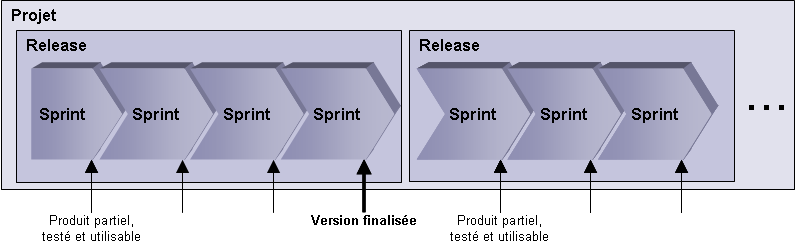
\includegraphics[width=\textwidth]{planification_scrum.png}
  \end{center}
  %% \caption{Exemple de planification Scrum}
\end{figure}

\clearpage
\subsection{Issues}
Avant de commencer un sprint, on lui associe une liste de fonctionnalités qui
devront être réalisées, tirées du backlog de produit (cf. Schéma Vue synthétique
du processus Scrum).\\
Ces fonctionnalités sont sélectionnées pour être implémentées dans ce sprint.\\

Chaque fonctionnalité est découpée par l'équipe en tâches élémentaires de
quelques heures et vont dans le backlog de sprint. Ces tâches élémentaires sont
appelées des \textbf{issues} et peuvent être consultées à tout moment par les
programmeurs.\\

L'image ci dessous présente la liste des issues qui m'ont été
assignées. \\
Chaque membre de l'équipe peut les consulter et y ajouter un
commentaire, pour discuter de l'implémentation ou pour proposer des
solutions possibles.

\begin{figure}[H]
  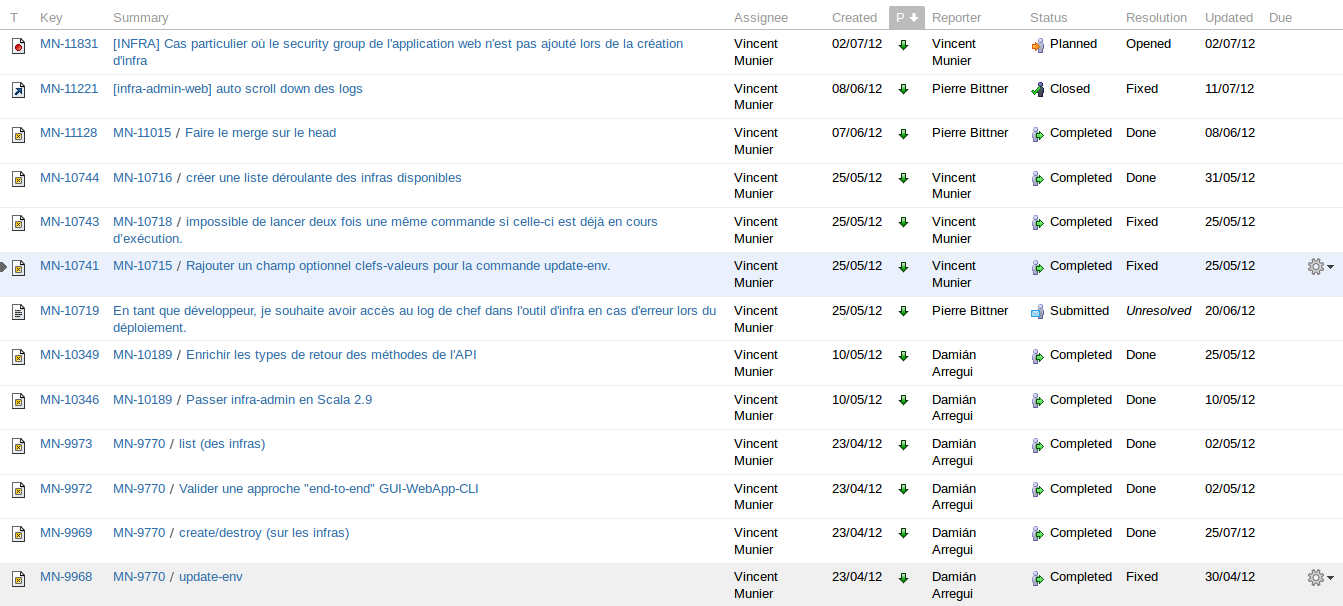
\includegraphics[width=\textwidth]{mes-issues.png}
  \caption{Liste des issues qui m'ont été assignées}
\end{figure}

\clearpage

Une issue est la description très courte d'un besoin utilisateur.\\
Dans l'exemple ci-dessous, nous pouvons retrouver les différentes informations
attachées à une issue. \\
Nous pouvons retrouver la date de création, le nombre d'heures estimé, le nombre
d'heures loguées et bien d'autres informations.\\

\begin{figure}[H]
  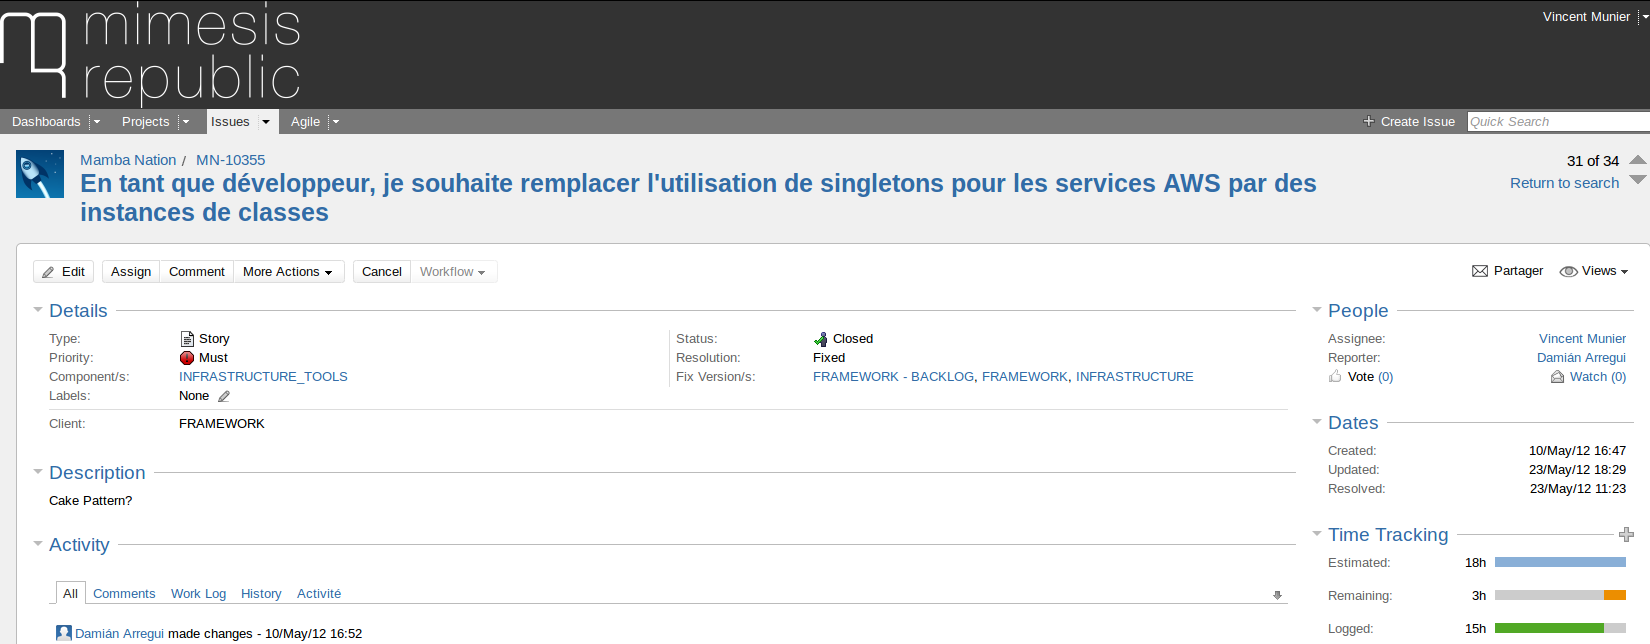
\includegraphics[width=\textwidth]{issue-MN-10355.png}
  \caption{Exemple d'issue qui m'a été attribué}
\end{figure}

Ce découpage de tâches de courtes durées est un des gros points forts de la
méthodologie agile Scrum.\\
En effet, il permet d'avoir un système testable qui peut être livré au client à
chaque instant. Bien sur, nous devons prévenir le client que telle
fonctionnalité n'est pas encore implémentée.\\
Mais le client peut ainsi nous faire des retours sur ce qu'il en pense, le plus
régulièrement possible.\\
En cas de problèmes, il est bien plus facile de faire des interventions rapides
que si le client donnait son avis tous les six mois.\\
Il peut également décider à tout instant de mettre son produit en production
s'il le souhaite.

\subsection{Réunions}
\subsubsection{Réunion chaque jour}
Chaque journée de travail commence par une réunion de 15 minutes maximum appelée
standup (Daily standup).\\

Le ScrumMaster donne la parole à chaque membre de l'équipe.\\
À tour de rôle,  nous devons répondre à 3 questions :
\begin{itemize}
\item Qu'est-ce que j'ai fait hier ?
\item Qu'est-ce que je compte faire aujourd'hui ?
\item Quelles sont les difficultés que je rencontre ?\\
\end{itemize}
L'équipe se met ensuite au travail, elle travaille dans une même pièce.

\subsubsection{Réunion entre deux sprints}
À la fin du sprint, tout le monde se regroupe pour effectuer une réunion qui se
déroule en deux étapes :
\begin{itemize}
\item La revue de sprint (sauf si c'est le premier sprint)
\item La planification du prochain sprint\\
\end{itemize}

La durée de cette réunion est d'environ quatre heures.\\\\
\textit{\underline{Revue du sprint précédent}}\\

Le Scrum Master commence par faire une présentation de ce qui était attendu pour
ce sprint.\\
Puis il énonce les fonctionnalités qui ont été réellement implémentées, groupées
par programmeur.\\
Le Scrum Master donne ainsi la parole à chaque membre de l'équipe, pour qu'il
donne un retour d'expérience, les tâches qu'il a accomplies avec succès, les
imprévus qu'il a rencontrés.\\\\
\textit{\underline{Planification du sprint à venir}}\\

La réunion de planification consiste à définir d'abord
un but pour le sprint, puis à choisir les fonctionnalités de produit qui seront
réalisées dans ce sprint. \\

Dans un second temps, l'équipe décompose chaque fonctionnalité de produit en
liste de tâches (items du backlog du sprint), puis estime chaque tâche en
nombre d'heures. 

\begin{figure}[H]
  \begin{center}
    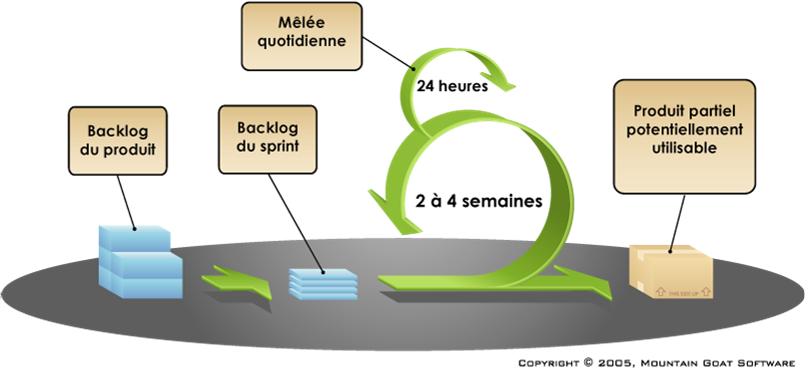
\includegraphics[width=\textwidth]{scrum.png}  
  \end{center}
  \caption{Vue synthétique du processus Scrum}  
  \label{scrumsynthese}
\end{figure}

\newpage
\subsection{Glossaire}

\begin{itemize}
\item[]\textbf{Backlog}

  Liste ordonnée de toutes les choses à faire. Il y a le backlog de produit qui
  énumère les exigences avec le point de vue du client et le backlog de sprint qui
  contient les tâches de l'équipe. \\

\item[]\textbf{Directeur de produit / Product owner}

  Le représentant des clients. Littéralement le propriétaire du produit.\\

\item[]\textbf{Release}

  Une release correspond à la livraison d'une version. Par habitude, on parle de
  release pour considérer la période de temps qui va du début du travail sur cette
  version jusqu'à sa livraison et qui passe par une série de sprints
  successifs. \\

\item[]\textbf{Scrum}

  Scrum c'est la méthode mais c'est aussi le nom usuel de la réunion quotidienne
  limitée à un quart d'heure. \\

\item[]\textbf{Sprint}

  Bloc de temps aboutissant à créer un incrément du produit potentiellement
  livrable. C'est le terme utilisé dans Scrum pour itération. Aux débuts de Scrum,
  un sprint durait 30 jours. La pratique actuelle est de 2 à 4 semaines.\\

\item[]\textbf{Scrum Master}

  Il dirige les réunions scrum. Il s'assure que le projet avance comme prévu.\\
\end{itemize}




      %% dernière relecture : 13 août

\chapter{Le contexte}
 %% : l'outil de déploiement du jeu en ligne
\section{Architecture de l'écosystème Mamba Nation}

\subsection{Architecture Générale}

Mamba Nation est composé de trois couches : La couche utilisateur, la couche
Game Server aussi appelée ``La Nation'', et la couche Back-Office.

La couche utilisateur est composée de l'application Facebook, l'applet qui
affiche le monde Mamba Nation en 3D, un site web, un forum et une application
IPhone appelée Battle.
L'applet est responsable du rendu 3D du jeu.

La Nation regroupe un ensemble de composants applicatifs qui donnent vie au
monde de la Nation: moteur du Jeu, base de données, etc.. Des Web services sont
aussi utilisés pour permettre aux partenaires externes d’accéder à la Nation.
Les services ``Event log'' sont un élément central qui collecte les événements
utilisateurs.

La couche Admin est composée de la BI (Business Intelligence Platform) qui
produit un grand ensemble de KPI (Key Performance Indicator) du jeu et un outil
Back-Office pour que le jeu puisse être géré par les équipes Operation.

\subsection{Diagramme Fonctionnel}

Le diagramme représente les principaux services fonctionnels de Mamba Nation.
Ces services peuvent être organisés en trois couches :
\begin{itemize}
\item couche User: services accessibles directement par l'utilisateur final
\item couche Game: moteur du jeu, les services pour les partenaires externes et les
  composants internes
\item couche Admin: reporting et outils de gestion
\end{itemize}

\begin{center}
\begin{figure}[H]
  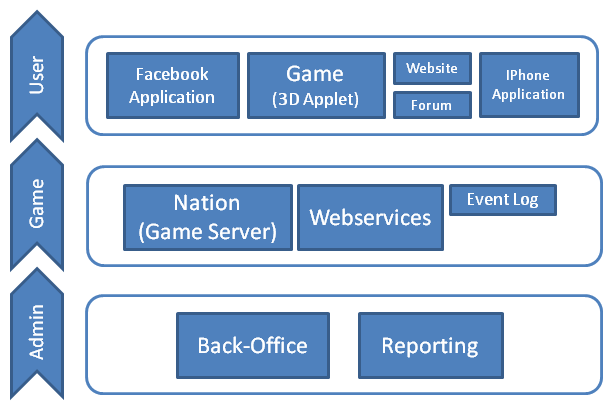
\includegraphics[scale=0.75]{MN-functional-diagram.png} 
  \caption{Diagramme fonctionnel de la Nation}
\end{figure}
\end{center}

\subsection{Architecture Technique}

La Nation contient les services de base de Mamba Nation. Ça inclut le Game
Server, le moteur d'applet 3D, l'application facebook, les services web et le
site web.

La Nation utilise aussi un ensemble de services techniques :
\begin{itemize}
\item Zookeeper : service centralisé pour maintenir les informations de configuration
\item Route 53 : service Web de système de noms de domaine (DNS)
\item Mongo DB : base de données orientée document
\item RabbitMQ : solution de messagerie orientée messages pour créer un réseau
  d'échange d'informations entre des applications.
\item RDS : base de données MySql fournie par Amazon
\item Jetty : moteur de servlet basé sur Java
\item Apache : héberge le site php
\item S3 : plateforme de stockage ``illimité''
\end{itemize}

Les utilisateurs se connectent au Game Server à travers les dispatchers qui ont la
responsabilité de gérer les connections TCP.

La plupart des services sont développés avec le langage Scala ce qui facilite le
développement d'applications évolutives.

Le site web est développé en PHP avec un serveur Zend et un cache APC. Il est
déployé sur Apache.

\begin{figure}[H]
  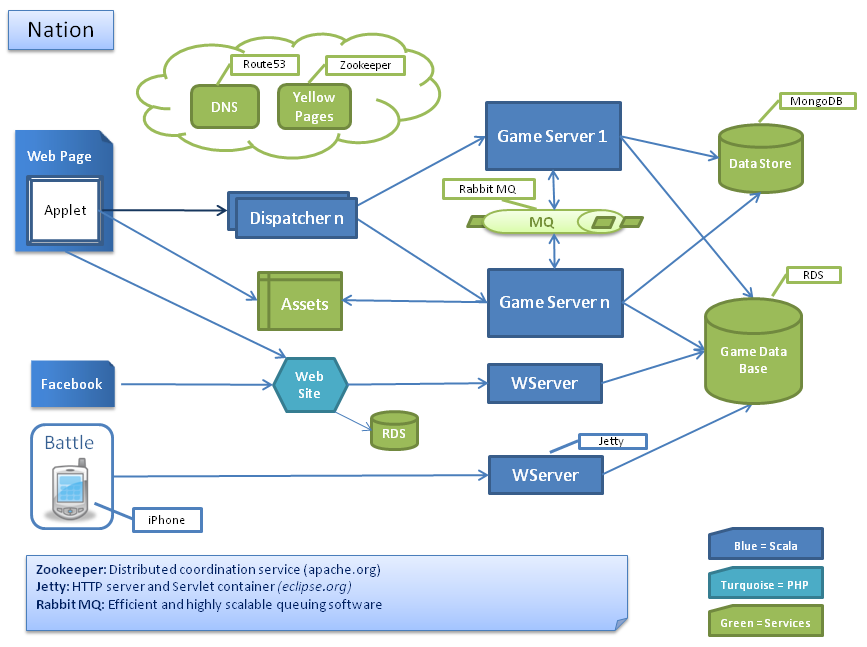
\includegraphics[scale=0.75]{MN-technical-diagram.png} 
  \caption{Diagramme technique de la Nation}
\end{figure}

\subsection{Statistiques du Jeu}

\begin{figure}[H]
  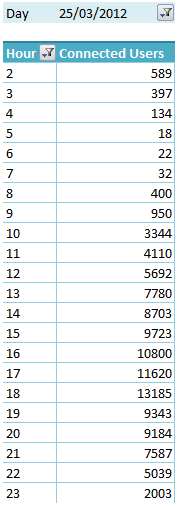
\includegraphics[width=0.20\textwidth]{connected-users-diagram.png}
  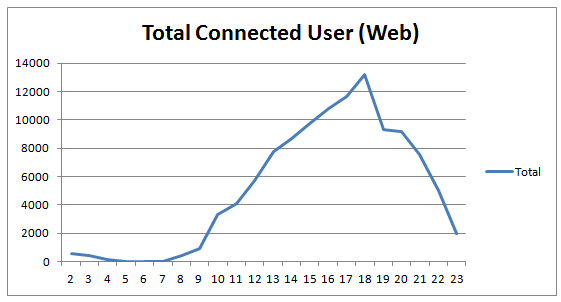
\includegraphics[width=0.80\textwidth]{connected-users-graph.png}
  \caption{Diagramme du nombre d'utilisateurs connectés dans la journée du 25 mars 2012}
\end{figure}

\section{L'outil d'infra : un outil pour déployer le jeu}

Les ingénieurs de l'équipe \textit{infrastructure} ont conçu un outil en ligne
de commande pour déployer une infrastructure.
Chaque équipe de l'entreprise utilise cet outil pour gérer leur propre
infrastructure. Par exemple, l'équipe \textit{engine} utilise cet outil de
déploiement pour gérer leur infrastructure \textit{engine}.

Un développeur de l'équipe \textit{engine} peut exécuter la commande
\textit{status engine} pour se renseigner sur l'état de son infra. L'outil en
ligne de commande affiche :
\begin{verbatim}
    engine_all_0 (i-51e60a18 / 54.247.21.95)        :       running
    Instance reachability check passed
    System reachability check passed
\end{verbatim}
Tout va bien, l'instance \verb?engine_all_0? est bien en train de s'exécuter.

L'objectif principal du stage est de créer une interface Web pour piloter cet
outil d'infra de déploiement du jeu en ligne sur le Cloud.

\section{Le concept de Promises}

L'outil d'infra utilise le concept de \textit{Promises} partout dans son code.

Les Promises fournissent un bon moyen de raisonner sur l'exécution de
nombreuses opérations en parallèle - d'une façon efficace et non bloquante.

L'idée est simple, une Promise est une sorte de conteneur d'objet que
l'on peut créer pour un résultat qui n'existe pas encore.

Généralement, le résultat d'une Promise est calculé de manière
concurrente et peut être récupéré plus tard.
Composer des tâches concurrentes de cette manière permet d'avoir du code
parallèle non bloquant, asynchrone plus rapide.

Une Promise est une abstraction qui représente une valeur qui peut devenir
disponible à un certain point.
Un objet Promise contient soit le résultat d'un calcul soit une exception dans
le cas où le calcul a échoué.
Une propriété importante d'une Promise est qu'elle est immuable; le détenteur de
la Promise ne peut à aucun moment modifier la valeur qu'elle contient.

Voici un exemple de création d'une Promise qui appelle une méthode getUsers de
façon asynchrone. Le résultat devient disponible une fois que la Promise se
termine.
\lstset{language=scala,
  frame=single                   % adds a frame around the code
}
\begin{lstlisting}
  val usersProm: Promise[List[Users]] = async {
    session.getUsers
  }
\end{lstlisting}

Nous pouvons chaîner les calculs sur la Promise de base en utilisant la méthode
map qui reçoit une fonction en paramètre.
\begin{lstlisting}
  val alexProm: Promise[User] = usersProm.map { users => users.filter(_.name == ``Alex'').head }
\end{lstlisting}

Une fois tous les calculs effectués sur notre Promise, nous pouvons récupèrer sa
valeur de façon bloquante (waitAndGetEither) ou non bloquante (mapEither).
Récupération de l'utilisateur Alex de façons bloquante :
\begin{lstlisting}
val alex:User = alexProm waitAndGetEither() match {
    case Right(alex: User) => alex
    case Left(t: Exception) => t.printStackTrace(); throw t
  }
\end{lstlisting}
Si la Promise s'est terminée avec succès alors la méthode waitAndGetEither
renvoie une instance Right qui contient notre utilisateur Alex.
Si l'une des fonctions passée aux différentes Promises de la chaîne a échouée, la
méthode waitAndGetEither renvoie une instance Left qui contient l'exception
lancée.

Les promises feront parties de la bibliothèque standard de Scala 2.10
(\url{http://www.scala-lang.org/node/12550}).

\section{L'outil d'infra et AWS}

L'outil d'infra utilise l'API Java AWS pour :
\begin{itemize}
\item créer, supprimer une instance
\item récupérer le status d'une instance
\item démarrer, arrêter une instance
\item créer, supprimer un groupe de sécurité
\item authoriser des IP et ports sur un groupe de sécurité
\item lister les groupes de sécurité
\end{itemize}

\section{L'outil d'infra et Chef}

Toutes les informations concernant une infra sont stockées dans Chef.
Lors de la création d'une infra, l'outil en ligne de commande stocke entre
autres le nom de l'infra, la région AWS, le nom de la base de données et le nom
du groupe de sécurité dans un Databag Chef.

L'outil d'infra utilise l'API REST de Chef pour récupérer des informations ou
effectuer des actions.

\section{Usage}

L'outil d'infra en ligne de commande reçoit en entrés un nom de commande
et ses arguments. Si la commande n'existe pas, l'outil d'infra affiche l'aide
d'usage.
Voici l'affichage de l'aide, on peut y voir toutes les commandes disponibles :
\begin{verbatim}
Usage: infra <cmd> [<infra>] [<file>] [<key>=<value>]*

    Infra admin tool config file:
      Config parameters must be specified in the 'infra.conf' file located in the 'config' directory.
      It should contain one <field>=<value> definition per line.

    Infra creation, pass config file:
      create <file>
        Create an infrastructure as defined in the given config file.
     migrate <file>
        Migrate databases for a particular environment in an infrastructure as
        defined in the given config file.


    Infra management, pass infra:
      start <infra>
        Start the given infrastructure.
      stop <infra>
        Stop the given infrastructure.
      status <infra>
        Show status of the given infrastructure.
      destroy <infra>
        Destroy the given infrastructure.

    Service management, pass infra:
      start-services <infra>
        Start services on the given infrastructure.
      stop-services <infra>
        Stop services on the given infrastructure.
      restart-services <infra>
        Restart services on the given infrastructure.
      status-services <infra>
        Show status of the services on the given infrastructure.

    Database management, pass infra:
      deploy-db <infra>
        Run the 'deployDb' command on the given infrastructure.
      liquibase-install <infra>
        Run the 'liquibase-install' command on the given infrastructure.
      liquibase-sync <infra>
        Run the 'liquibase-sync' command on the given infrastructure.
      liquibase-update <infra>
        Run the 'liquibase-update' command on the given infrastructure.
      run-migration-tool <infra>
        Run the 'run-migration-tool' command on the given infrastructure.

    Text management, pass infra :
      deploy-wti <infra>
        Export the last texts from WTI on amazon S3 ; to really use them you
        have to modify the file "launch.js.php" on the "a" environment.


    Environment management, pass infra and optionally updated values:
      show <infra> [<key>]*
        Show the "a" environment on the given infrastructure.
      update-env <infra> <file>
        Update the "a" environment on the given infrastructure as defined in the given config file.
      update-env <infra> [<key=value>]*
        Update the "a" environment on the given infrastructure as defined in the key-value arguments.

    Various utilities, rarely used:
      list
        List all infrastructures.
      start-all
        Start all infrastructures and all services.
      stop-all
        Stop all infrastructures.
      register-dns <infra>
        Register DNS records for the given infrastructure.
      switch-dns <infra>
        Switch LIVE dns to point to the given infrastructure.
      export <infra>
        Export the databag item describing the given infrastructure from the Chef server to a file.
      import <infra>
        Import the databag item describing the given infrastructure from a file to the Chef server.
      export-databags
        Export all databags from the Chef Server to the file system.
      import-databags
        Import all databags from the file system to the Chef Server.
\end{verbatim}



      
\chapter{Mes réalisations}

\section{Présentation du framework Play!}

Play! est un jeune framework qui permet de créer facilement des
applications web avec Java et Scala.
Mon stage a deux buts majeurs pour l'entreprise :

\begin{enumerate}
\item Rendre accessible à tous l'utilisation de l'outil d'infra en proposant
  une interface web ergonomique.
\item Explorer le potentiel du framework Play! pour qu'il remplace
  éventuellement du code php existant dans différents logiciels de
  l'entreprise.
\end{enumerate}

Durant mes deux premières semaines de stage, j'ai préparé des slides pour une
présentation du framework. Cette présentation met en avant les caractéristiques
de Play!, ses points forts et faiblesses, et comment il se place face aux
alternatives existantes.
L'équipe croit au potentiel du framework mais attend le résultat de
l'interface web de l'outil d'infra pour décider de remplacer le code php
existant.

\underline{\textit{Bilan}} : Cette présentation m'a permis de travailler
l'aisance orale devant un public de techniciens. J'ai pu confronter mes arguments
en faveur (ou défaveur) du framework Play! avec ceux d'autres programmeurs
expérimentés qui ont déjà utilisé plusieurs frameworks Web.

\noindent\hrulefill

La semaine suivante consiste à tester l'outil d'infra en ligne de
commande et à réfléchir à l'interface utilisateur pour l'application web (url
disponibles, dispositions des boutons et des champs de saisies).

Une nouvelle branche est ajoutée dans Mercurial pour accueillir l'application web.
Le développement peut commencer!

\section{Le déploiement}

Le déploiement doit être fonctionnel avant de développer l'application.

En effet, il se peut que les contraintes d'infrastructure empêchent
le déploiement d'une application : l'espace disque dur qui peut être insuffisant
pour accueillir l'application, l'impossibilité d'ouvrir des ports http.
Si on ne sait pas mettre à disposition une application à ses
utilisateurs (i.e. la déployer) le travail réalisé est inutile, elle n'apporte
aucune valeur.
Nous devons donc vérifier que le déploiement fonctionne bien de bout en bout.

Pour cela, une application simpliste est créée.
Elle affiche juste une page web avec du contenu statique.
Il faut maintenant héberger l'application puis automatiser le déploiement en
programmant des scripts.

\subsection{Amazon héberge l'application}

Sur Amazon Web Services, une instance EC2 portant le nom 'infra-admin-web' est
créée. C'est en fait le serveur qui hébergera l'application. Le
système d'exploitation de cette instance est Ubuntu 12.04 .
C'est une instance de type \textit{t1.micro} qui est idéale pour le type
d'application web attendue.
En effet, les clients de l'application web seront les membres de la société.
Du fait du nombre limité d'utilisateurs, environ 25 développeurs,
une puissance CPU limitée suffit.

Une instance Micro (\textit{t1.micro}) fournit une petite quantité de ressources CPU
constantes et augmente dynamiquement sa capacité CPU sur de courtes durées
lorsque des cycles supplémentaires sont disponibles. Donc elle convient bien
aux applications à moindre trafic ou aux sites consommant un nombre de cycles
significatif périodiquement.

Le schéma suivant illustre l'utilisation CPU typique d'une application web
tournant sur une instance de type \textit{t1.micro} :
\begin{figure}[H]
  \begin{center}
    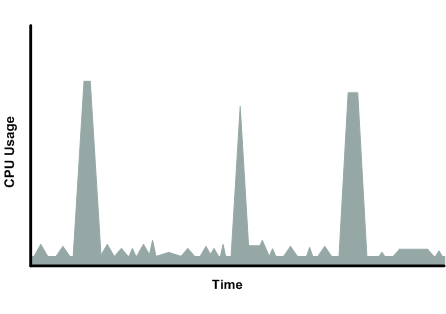
\includegraphics[scale=0.8]{cpu-usage.png} 
  \end{center}
  \caption{utilisation CPU pour une instance du type micro}
\end{figure}

Les instances de type micro sont aussi les moins chères de tous les types
d'instances proposés par Amazon. Leurs prix est de seulement 2 centimes de
dollars par heure.

\underline{\textit{Bilan}} : Découverte et première utilisation d'AWS. Ce
service de Cloud Computing fourni par Amazon est l'investissement le plus
rentable pour les jeunes entreprises. De plus en plus d'entreprises l'utilisent
car il est économique, fiable et évolutif. Avoir les droits d'accès pour piloter
AWS est une opportunité pour moi d'apprendre à maîtriser cet outil.

\subsection{Scripts Bash}

Maintenant que nous disposons d'une instance EC2 réservée pour l'application
web, il faut automatiser les actions récurrentes qui devront être effectuées.

Quatre scripts Bash sont créés pour exécuter les tâches récurrentes :
deploy.sh, start.sh, stop.sh et restart.sh pour respectivement déployer
l'application web, la démarrer, l'arrêter et la redémarrer.

deploy.sh est un script qui se trouve sur la machine local.
Ce script package l'application puis la copie sur l'instance EC2 via scp.
Les scripts start.sh, stop.sh et restart.sh se trouvent sur l'instance EC2 et
peuvent être appelés à distance via ssh.

\underline{\textit{Bilan}} : Mes connaissances en Bash et sur l'environnement
Linux m'ont permis de créer rapidement ces scripts d'automatisation de
déploiement.

\section{Premier concept de webapp : appeler l'outil d'infra comme une commande
  shell}
\noindent Les objectifs de la première version de la webapp sont les suivants :
\begin{enumerate}
\item La webapp exécutera l'outil d'infra en ligne de commande comme un
  programme externe.
\item La webapp doit permettre d'exécuter deux commandes en parallèle.
\end{enumerate}

Le code côté serveur est écrit en Scala.
Puisque toute classe Java peut être naturellement instanciée dans du code Scala,
c'est la classe Java ProcessBuilder qui est utilisée pour exécuter
l'outil d'infra comme programme externe.
Qu'en au code côté client, il doit afficher la sortie de la commande dans le
navigateur.

Une contrainte apparaît :
Certaines commandes de l'outil d'infra prennent beaucoup de temps à s'exécuter.
L'output de la commande doit donc être affichée au fur et à mesure de son
exécution. Pour ce faire :\\
\textit{Côté serveur}, un BufferedReader récupère dynamiquement la sortie de la commande.\\
\textit{Côté client}, du JavaScript affiche progressivement le résultat.

Le point restant est la communication entre le serveur et le navigateur du
client pour afficher dynamiquement du contenu dans la page web.

\subsection{Communications asynchrones pour une application web temps réel}
%\textit{\underline{Communications asynchrones pour une application web temps réel}}\\

Dans une application Web traditionnelle, lorsque l'utilisateur effectue une
action, celle-ci est exécutée et le navigateur attend le résultat pour rendre
la main à l'utilisateur. Lorsque cette action requiert un calcul coûteux
au serveur, cela occasionne des délais et une attente pour le client.

Le mode asynchrone élimine cette attente. Les requêtes au serveur sont lancées
sans que soit suspendue l'interaction avec le navigateur et la page est mise à
jour lorsque les données requises sont disponibles.

La première solution bien connue pour disposer de ce comportement asynchrone est
\textit{Ajax}.
\textit{Ajax} est une technologie permettant de créer des applications qui simulent un
comportement temps réel. Le navigateur envoi une requête HTTP à intervalle
régulier et reçoit une réponse.
Il existe aujourd'hui des alternatives à \textit{Ajax} pour voir des données se
mettre à jour dans sa page web sans appuyer sur le bouton refresh.

La webapp de l'outil d'infra utilise des \textit{WebSocket}.
C'est une autre technologie web, bien plus récente, qui permet de créer de vrais
applications temps réel.
Alors que le protocole HTTP opère par une succession de requêtes et réponses
alternatives, \textit{WebSocket} est bidirectionnel : une connexion statique s'établit
entre le serveur et le client et les deux parties envoient des données à leur
convenance.
C'est un authentique canal de communication bidirectionnel (push depuis le
serveur) transparent pour les firewalls, proxy, et routeurs.
Il n'y a aucune latence réseau lors des transmission, les performances réseaux
qu'elle offre est l'un de ses gros points forts.
Le framework Play! fournit une bibliothèque complète pour utiliser les
\textit{WebSockets}.
La webapp fait donc usage des \textit{WebSockets} pour récupérer dynamiquement le
résultat de la commande et l'afficher dans le navigateur.

Pour chaque nouvelle page ouverte, une WebSocket est créée.
Deux utilisateurs peuvent alors exécuter leur commande en parallèle sans
blocage ni intercalage des logs des commandes.

Voici une capture d'écran de l'interface web disponible avec la première version
de la webapp :
\begin{figure}[H]
  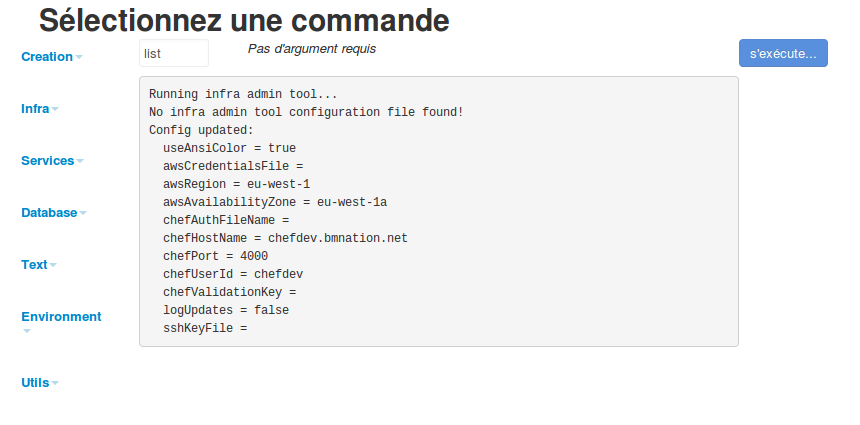
\includegraphics[width=\textwidth]{webapp-processbuilder.png}
  \caption{Exécution de la commande ``list'' avec la première version de la webapp}
\end{figure}

\underline{\textit{Bilan}} :
\begin{itemize}
\item Le développement est rapide avec Play!. Le rechargement à
  chaud de l'application et l'utilisation du langage évolué Scala permettent de
  gagner beaucoup de temps.  
\item Les interactions côté client se font en JavaScript et
  je gagne en aisance à programmer avec ce langage que je connais à peine.
\item  Découverte des WebSocket, cette technologie de dialogue client/serveur
  bidirectionnelle ouvre de belles perspectives à de nouvelles fonctionnalités
  Web.
\end{itemize}

\section{Transformer l'outil d'infra en bibliothèque}

\underline{\textit{La demande}} : Transformer l'outil d'infra en bibliothèque pour ne plus
lancer un processus séparé et donc une JVM à chaque exécution de commande.
Mais, très important, l'outil doit toujours fonctionner en ligne de
commande.

\underline{\textit{L'objectif}} : Générer un jar de l'outil d'infra pour ensuite
l'intégrer à l'application web. Les méthodes de l'outil d'infra seront
directement accessibles dans le code source de la webapp.

La transformation de l'outil d'infra en API impose plusieurs changements qui
sont présentés dans les sous-sections qui suivent.

\subsection{Des singletons transformés en simples classes}

Toutes les classes étaient des services. Elles étaient toutes des singletons.
Les services proposent des méthodes utilitaires et n'ont pas d'état. Il était
donc logique d'avoir des singletons car nous n'avions pas besoin de plus d'une
instance par service. 

De même, il existait un singleton Logger qui était utilisé par tous les autres
singletons afin de logguer leurs différentes actions.

Dans l'outil d'infra en ligne de commande, un seul logger suffisait, un simple
logger qui enregistre tout dans un fichier.
Mais pour que l'outil se transforme en API, l'utilisateur doit avoir le
contrôle sur le logger. L'utilisateur doit pouvoir choisir son logger, il doit
pouvoir en utiliser plusieurs si il souhaite.

C'était en effet le cas de l'application web qui allait être le premier
programme à utiliser l'API. L'application web a besoin de plusieurs
loggers. En fait, elle a besoin d'un logger par internaute.
Une nouvelle instance du Logger est créée pour chaque nouvel internaute afin
que les résultats des commandes lancées par un internaute soient isolés dans son
propre fichier. Les logs des internautes ne doivent pas être mélangés.

Un refactoring important a permis la transformation de l'outil d'infra en API.
Tous les singletons sont transformés en simples classes.
Puisqu'il n'existe plus de singleton, les constructeurs de ces classes prennent
alors en paramètre les instances d'autres classes dont elles dépendent.

Par chance, l'outil d'infra a été développé avec un langage statiquement
typé, Scala en l’occurrence.
Lorsqu'un singleton se transforme en simple classe, le code extérieur qui
utilisait ce singleton doit changer sa façon de l'appeler.
Grâce au typage statique, Eclipse affichait les erreurs de compilation dans
les différents fichiers faisant usage de la classe modifiée. Il suffisait alors
de suivre ces erreurs et de les corriger.

\underline{\textit{Bilan}} : Cette tâche fut assez longue à faire mais il n'y
avait pas de complexité particulière, le résultat était assuré.
En plus de l'objectif premier qui était de pouvoir utiliser l'outil d'infra en
tant qu'API, les dépendances entre les classes sont maintenant clairement
exposées ce qui facilite la compréhension du code.

\subsection{Libération mémoire du cache}

L'outil faisait aussi utilisation d'un cache pour l'optimisation de méthodes
appelées plusieurs fois durant l'exécution d'une même commande.

Puisque ce programme était conçu pour exécuter une seule commande, la
consommation mémoire de ce cache ne posait pas problème.
À la fin de l'exécution de la commande, le programme se termine et la JVM
se charge de libérer la mémoire allouée.

Dans le cadre d'une API, le problème est différent. Le client qui utilise l'API
de l'outil d'infra ne souhaite peut-être pas exécuter une seule commande.
Si le client exécute plusieurs commandes successives, le cache grossit pour
chaque nouvelle commande exécutée et consomme de plus en plus de mémoire.

C'est le cas de l'application web dont la durée d'exécution est \textit{supposée}
infinie. Une fois mise en production, l'application web doit être
continuellement disponible pour les utilisateurs. Seul le déploiement d'une
nouvelle version de l'application web doit engendrer son redémarrage.

Pour corriger ce problème, les données relatives à une commande sont supprimées
du cache lorsque l'exécution de cette commande se termine.

\underline{\textit{Bilan}} : Ce problème de cache non libéré n'a été détecté
qu'une fois l'application web mise en ligne. Après quelques jours
d'utilisation, une exception java.lang.OutOfMemoryError avait été lancée par la
JVM du serveur. Ce problème ne s'est pas reproduit une fois la solution mise en
place. L'option -XX:+HeapDumpOnOutOfMemoryError a aussi été rajouté au lancement
de la JVM pour récupérer à l'avenir une description complète de l'état du tas
(heap) de la mémoire si une même exception se produisait.

\clearpage
\subsection{Des types de retour plus riches}

Plusieurs méthodes de haut niveau, directement appelées par le main de l'outil
d'infra, ne renvoyaient rien car le seul retour utile était imprimé
sur stdout et stderr. Ces méthodes de haut niveau font maintenant parti de l'API
de l'outil d'infra et peuvent être appelées en dehors du main par n'importe
quelle autre méthode.
Les types de retour des méthodes de l'API ont donc été enrichis.

Par exemple, la commande 'list' affiche sur la sortie standard la liste de
toutes les infrastructures existantes.
Son type de retour était Unit (void en Java) et devient Seq[Infra] (en Java, le
type le plus proche serait List<Infra>).
Le client de l'API peut alors se servir de la liste des infrastructures retournée.

\underline{\textit{Bilan}} : L'application web utilise le jar de l'outil d'infra
pour accéder à ses méthodes. Il n'est plus nécessaire de lancer un processus
séparé pour exécuter une commande.

\section{Les pages de la nouvelle webapp}
L'application web possède trois pages :
la page \textit{Commands}, la page \textit{Infras} et la page \textit{History}.

\subsection{La page Commands}

C'est la page principale du site. C'est aussi la plus utilisée car c'est à
travers cette page qu'il est possible d'exécuter n'importe-quelle commande de
l'outil d'infra. 

\begin{figure}[H]
  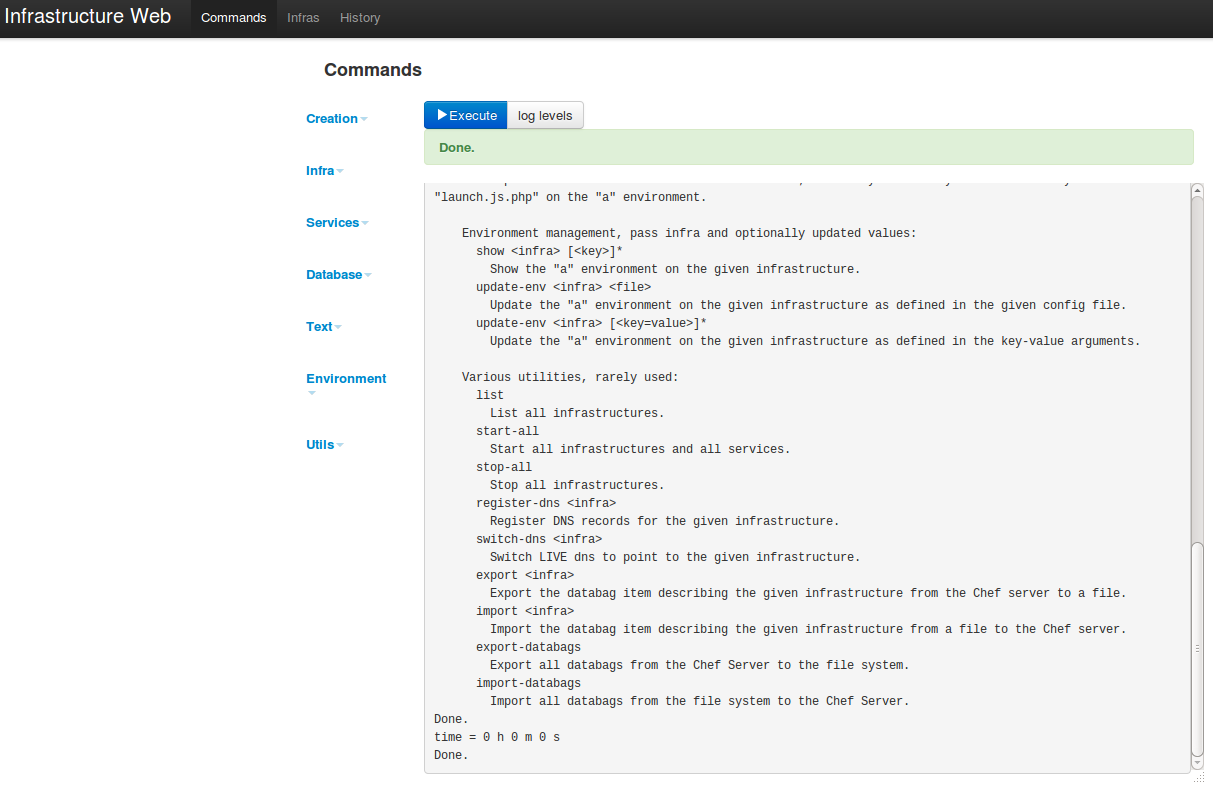
\includegraphics[width=\textwidth]{commands.png}  
\end{figure}

\clearpage
\vspace*{1cm}

\subsection{La page Infras}

La page Infras est un tableau de bord des infrastructures existantes.

Les informations exposées sont sont celles de l'outil d'infra. Tous les
attributs ne sont pas exposés à l'utilisateur. Si l'utilisateur souhaite
consulter l'ensemble des attributs d'une infrastructure, il peut le faire en se
connectant sur Chef car c'est Chef qui stocke toutes les informations relatives
à une infrastructure.

Le chargement des attributs pour l'ensemble des infrastructures existantes met
environ 5 secondes à s'exécuter sur l'instance EC2 qui héberge la webapp.
Un icône animé de chargement indique à l'utilisateur de patienter.

\begin{figure}[H]
  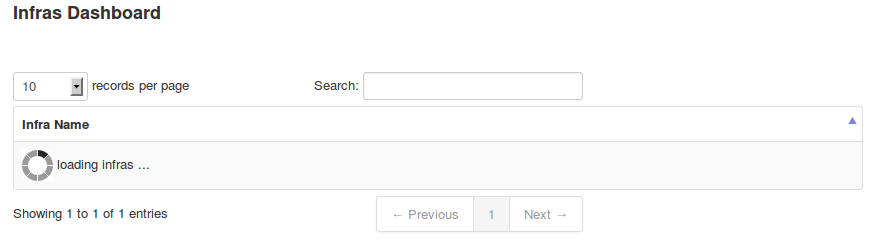
\includegraphics[width=\textwidth]{infras-dashboard-loading.png}  
  \caption{Chargement des infrastructures}
\end{figure}

\clearpage
Une fois les informations des infrastructures chargées, tous les noms d'infra
sont affichés sous forme de tableau.
\begin{figure}[H]
  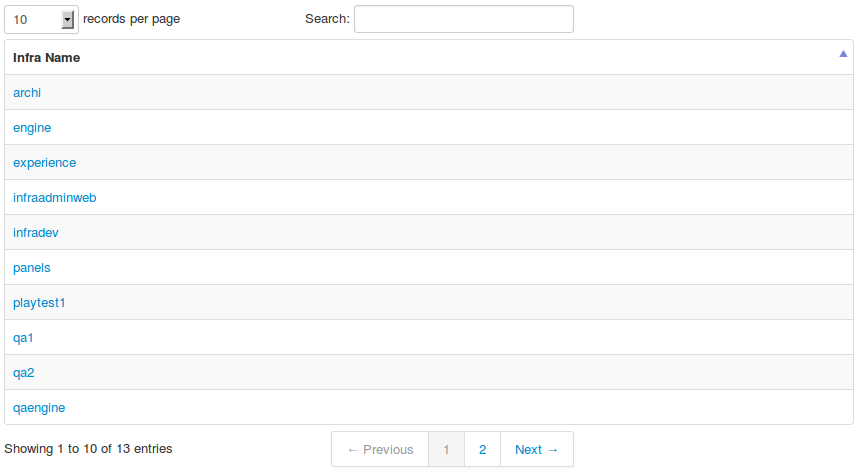
\includegraphics[width=\textwidth]{infras-dashboard.png}  
  \caption{les noms d'infrastructure présentés dans un tableau}
\end{figure}

L'utilisateur peut cliquer sur l'infrastructure qui l'intéresse.
Un deuxième tableau se présente à l'utilisateur dans lequel il peut consulter
les versions des différents services de l'infrastructure sélectionnée.
\begin{figure}[H]
  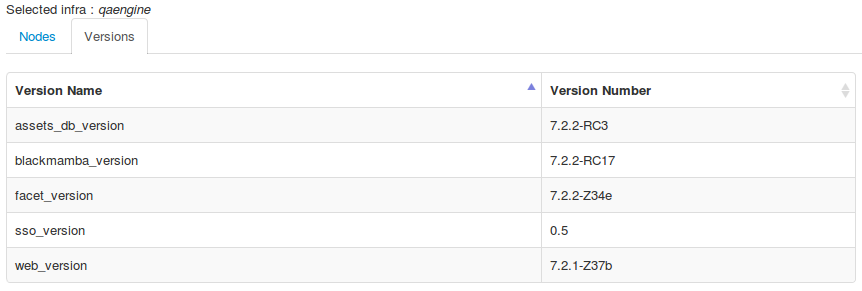
\includegraphics[width=\textwidth]{infra-versions.png}  
  \caption{les versions des services de l'infrastructure qaengine}
\end{figure}

\clearpage
Les nœuds appartenant à l'infra sélectionnée sont aussi accessibles via un
onglet \textit{Nodes}. 
Ce tableau nous affiche des informations intéressantes pour chaque nœud telles
que l'ID de l'AMI (Amazon Machine Image), le type d'instance EC2 qui héberge le
nœud, le hostname que l'on peut utiliser si on souhaite se connecter en ssh sur
l'instance du nœud, et enfin la liste des Security Groups.

\begin{figure}[H]
  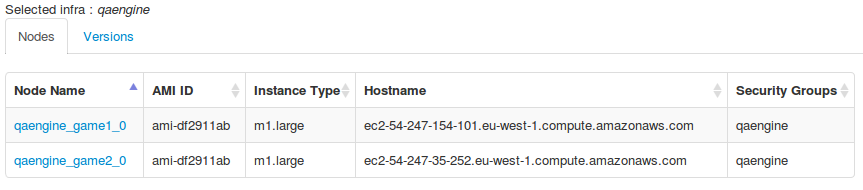
\includegraphics[width=\textwidth]{infra-nodes.png}  
  \caption{les nœuds de l'infrastructure qaengine}
\end{figure}

\bigskip
L'utilisateur peut cliquer sur le nœud qui l'intéresse.
Un troisième et dernier tableau se présente à l'utilisateur dans lequel il peut
consulter les rôles Chef appliqués au nœud sélectionné.

\begin{figure}[H]
  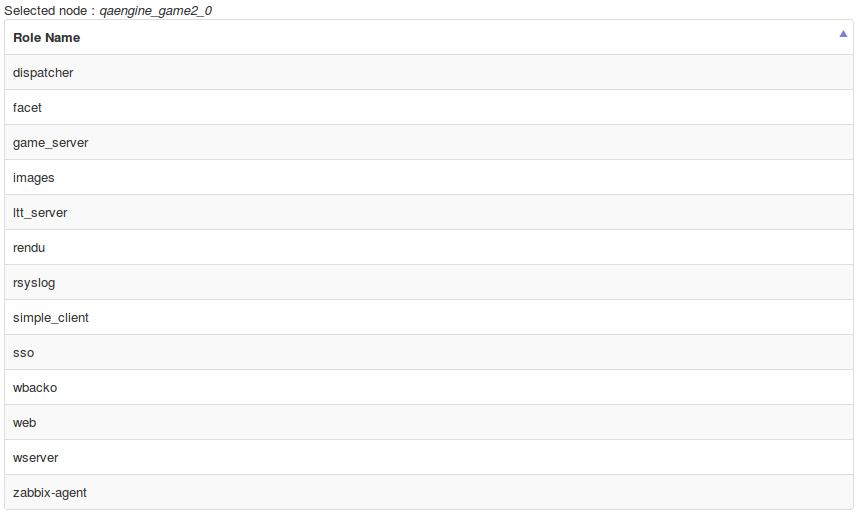
\includegraphics[width=\textwidth]{node-roles.png}  
  \caption{Les rôles du nœud qaengine\_game2\_0}
\end{figure}

\clearpage
\subsection{La page History}

La page History affiche l'historique des commandes exécutées.
Les 100 dernières commandes sont présentées dans un tableau dans l'ordre
chronologique inverse de leur date d'exécution, en commençant par l'exécution de
la commande la plus récente.
Ces 100 commandes ne sont pas persistées en base de données. Elles sont stockées
dans une file. Lorsqu'une 101 ème commande est ajoutée à la file, la première
est supprimée afin de ne conserver que les 100 dernières commandes. Cet élément
supprimé de la file sera récupéré par le garbage collector.
À l'avenir, il est prévu de rajouter la notion d'utilisateur avec un système
d'authentification, afin d'avoir un audit complet.

Cette page affiche deux informations supplémentaires qui sont le nombre de
pages \textit{commands} actuellement ouvertes (lorsqu'on déploie une nouvelle
version, on prévient par mail le nouveau déploiement et on vérifie que le nombre
de pages \textit{commands} ouvertes vaut 0) et le nombre de commandes
actuellement en cours d'exécution.

\begin{figure}[H]
  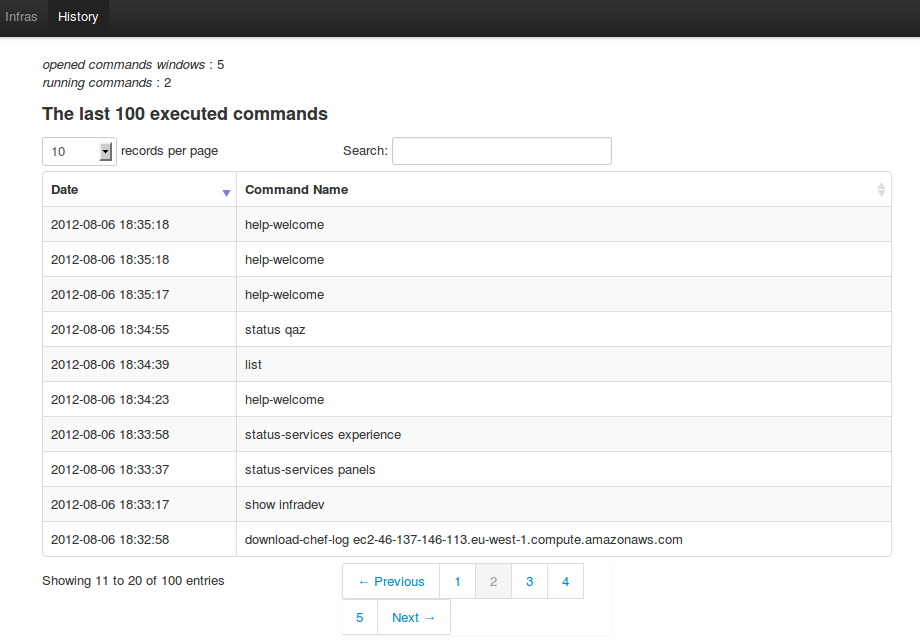
\includegraphics[width=\textwidth]{history.png}  
  \caption{Historique des 100 dernières commandes exécutées}
\end{figure}

\clearpage
\section{Composants de la page commands}

La webapp propose 30 commandes réparties dans 7 catégories différentes.
Voici un tableau récapitulatif de ces commandes.\\\\
\begin{tabular}{|c|c|c|c|c|c|c|c|c|c|c|c|}
  \hline
  \begin{bf}Catégories\end{bf} & \multicolumn{5}{c|}{\begin{bf}Commands\end{bf}} \\
    \hline
    Creation & create & migrate \\
    \cline{1-5}
    Infra & start & stop & status & destroy \\
    \cline{1-5}
    Services & start-services & stop-services & restart-services & status-services \\
    \cline{1-5}
    \multirow{2}*{Database} & deploy-db & liquibase-install & liquibase-sync\\
    \cline{2-4}
    & liquibase-update & run-migration-tool  \\
    \cline{1-3}
    Text & management & deploy-wti \\
    \cline{1-4}
    Environment & show & update-env-file & update-env \\
    \cline{1-6}
    \multirow{3}*{Utils} & help & free & list & start-all & stop-all \\
    \cline{2-6}
    & register-dns & switch-dns & export & import & export-databags\\
    \cline{2-6}
    & import-databags \\
    \cline{1-2}
\end{tabular}


\subsection{Champs de saisie}

%% \begin{figure}[H]
%%   \begin{center}
%%     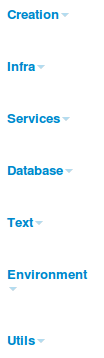
\includegraphics[scale=0.5]{categories.png} 
%%   \end{center}
%%   \caption{Les 7 catégories de commandes qui sont des listes déroulantes} 
%% \end{figure}

Lorsque l'utilisateur clique sur l'une des commandes d'une catégorie, il voit
apparaître en haut de l'application plusieurs champs de saisie qui décrivent les
arguments que doit recevoir la commande.
Il y a un champ de saisie pour chaque argument.
La commande \textit{restart-services} prend le nom d'une infra en
arguments. Elle possède donc un champ ``infra...''.
La commande \textit{update-env-file} prend le nom d'une infra et le chemin du
fichier de description de mise à jour de l'infra en arguments. Elle possède donc
un champ ``infra...'' et un sélecteur de fichier.

\begin{figure}[H]
  \begin{center}
    
\includegraphics[scale=0.5]{champ-update-env-file.png} 
  \end{center}
  \caption{Commande update-env-file} 
\end{figure}

\underline{\textit{Bilan}} : Ce nombre conséquent de commandes implique d'avoir
une grosse quantité de code HTML pour disposer tous les champs sur la
page web. Play! propose un système de templating qui permet de créer des
fonctions qui génèrent du code HTML depuis le serveur et permet d'éviter la
duplication de code. Le code ainsi créé est plus compact, plus facile à
comprendre et à maintenir.

\subsection{Sélecteur de fichier}

Un sélecteur de fichier est ajouté pour les commandes \textit{create},
\textit{migrate} et \textit{update-env-file} de l'outil d'infra.

Lorsque l'utilisateur clique sur le bouton 'Execute', le fichier sélectionné est
uploadé vers le serveur et la commande elle-même est exécutée côté serveur 
en utilisant le fichier qui vient d'être téléchargé.
Du code Ajax est utilisé pour ne pas avoir besoin de recharger la page lors de
l'envoie du fichier.
Ainsi le client peut recevoir l'output de la commande dans la page web.

\underline{\textit{Bilan}} : L'utilisation des \textit{WebSocket} est inadaptée
pour uploader un fichier. \textit{Ajax} convient parfaitement pour ce type de
tâche. Il fallait tout de même faire attention à ce que la commande ne soit
exécutée qu'une fois le fichier complètement téléchargé.

\section{Restructuration du code JavaScript}

La quantité de code JavaScript est devenue conséquente. Une restructuration du
code s'impose pour améliorer sa lisibilité, simplifier sa maintenance et
faciliter l'ajout de nouvelles fonctionnalités.

%% liens pour remplir les sous section RequireJS et CoffeeScript 
%% http://www.techno-science.net/?onglet=glossaire&definition=5410
%% http://pullrequest.org/2012/01/04/requirejs.html
%% http://yannesposito.com/Scratch/fr/blog/2011-01-03-Why-I-sadly-won-t-use-coffeescript/


\subsection{RequireJS}

Dans un langage de programmation comme Java, on ne se soucie pas du chargement
des dépendances. Il suffit de les définir (import java.utils.Collection par
exemple) et la JVM s'occupe de charger les modules de façon complètement
transparente pour le développeur.

Au contraire de ces langages évolués, la gestion des dépendances n'est pas
une tâche simple en JavaScript.
JavaScript ne possède pas de système de modules intelligent, ce qui rend le
découpage de code difficile.

Prenons un exemple. Les dépendances sont représentées comme des flèches du
module du client à gauche jusqu'au module requis à droite :

module1 $\rightarrow$ module2 $\rightarrow$ module3, module4 

En JavaScript, à chaque fois que module1 est utilisé, tous les autres modules
doivent être importés dans le bon ordre de la façon suivante :
%% mettre balise de code JavaScript à la place
\lstset{language=XML}
\begin{lstlisting}
  <script type="text/javascript" src="module4"></script
  <script type="text/javascript" src="module3"></script>
  <script type="text/javascript" src="module2"></script>
  <script type="text/javascript" src="module1"></script>
\end{lstlisting}

Heureusement, il existe quand même des moyens de définir de telles hiérarchies de
dépendances en JavaScript. RequireJS est une bibliothèque qui rend possible la
définition de dépendances entre modules de manière appropriée pour le navigateur.
RequireJS est une sorte de \#include/import/require pour JavaScript.\\
Voici un extrait de code de l'application utilisant RequireJS :
\lstset{language=JavaScript}
\begin{lstlisting}[caption=Définition du module commands avec RequireJS]
  define(
  // La liste des dépendances 
  // en python: import jquery, bootstrap-typeahead, bootstrap-button, bootstrap-dropdown
  ['jquery', 'bootstrap-typeahead', 'bootstrap-button', 'bootstrap-dropdown'], 
  function(dollar) { 
    // RequireJS assure que les quatre dépendances seront chargées et accessibles à
    // l'intérieur de la fonction.
    
    // définition de la fonction commands
    function commands(webSocketURL, listInfrasSocketURL) = {
      ...
    }
    
    // Utilisation du return pour exporter la fonction commands.
    // Tout ce qui n'est pas exporté reste privé au module.
    return commands;
  }
\end{lstlisting}


%% // in python: import myModule1, myModule2
%% requirejs(['myModule1', 'myModule2'], function (m1, m2) {


\subsubsection{Bénéfique pour la qualité du code}

\textit{\underline{Des APIs et namespace plus propres}}\\

La définition de modules avec RequireJS force le développeur à réfléchir à la
façon dont le module va partager les variables. Forcer le développeur à décider
ce qu'il veut exposer et quels sont les détails d'implémentation spécifiques
qui doivent être cachés conduisent à une meilleure encapsulation du code.

En plus, lorsque le développeur importe un module avec RequireJS, les propriétés
et méthodes exportées par le module sont accessibles à travers une variable
``package''. Ça permet à deux modules différents d'exporter un attribut avec le
même nom sans que l'un d'eux ne cache la valeur de l'autre.

%% http://imediava.wordpress.com/
%% http://imediava.wordpress.com/2012/04/23/intro-require-js/

\subsubsection{Bénéfique pour les performances}

\textit{\underline{Charger de plus petites ressources avec moins de requêtes}}\\

Deux principaux facteurs affectent le chargement d'une page :
\begin{itemize}
\item La taille des ressources. Le temps de chargement augmente avec la taille
  des ressources.
\item Le nombre de ressources. Plus il y a de ressources plus le nombre de
  requêtes augmente.
\end{itemize}

La meilleur approche pour gérer le premier cas est de ``minifier'' le code.
Minifier consiste à supprimer tous les caractères du code qui sont seulement
utiles pour rendre le code plus lisible (des espaces et retours à la ligne
entre autres).

Pour diminuer le nombre de requêtes HTTP, la solution habituelle (sans rentrer
dans la mise en cache) est de regrouper tous les fichiers dans un seul sans
modifier le code. De cette manière, le nombre de requêtes requises pour
récupérer les ressources du serveur est réduit à une seule.

RequireJS fournit un outil pour automatiquement minifier et
regrouper tous les modules en un seul. Cet outil est capable de minifier chaque
fichier CSS du projet et minifier et regrouper tous les fichiers JavaScript dont
les dépendances ont été définies en tant que module RequireJS.

\underline{\textit{Bilan}} : L'utilisation de \textit{RequireJS} était devenu
indispensable sans quoi la gestion des dépendances serait devenue un vrai
labyrinthe. Il est tout de même dommage de ne pas disposer de système de package
en JavaScript et de devoir faire recours à des bibliothèques tierces.

%% Peut-être ne pas mettre de section CoffeeScript ça fera trop de technologies
%% auxquelles je parle
\subsection{CoffeeScript}

Pour éviter de retomber dans les nombreux pièges rencontrés au cours du
développement de la partie cliente en JavaScript, j'ai décidé d'utiliser
CoffeeScript à la place de JavaScript.

CoffeeScript est un langage influencé par ruby qui fournit, entre autres choses,
les compréhensions de listes, une meilleure gestion des variables sans polluer
le namespace et plein d'autres outils qui rendent le développement JavaScript
plus simple. CoffeeScript compile vers du JavaScript lisible et bien formaté,
ce qui facilite le débugage.
Tout le code JavaScript écrit jusqu'ici est traduit en CoffeeScript.
Le code est plus concis (gain de $\sim$15\% pour le nombre de lignes de code) et le
développement plus fluide.

\underline{\textit{Bilan}} : CoffeeScript rend l'écriture de Javascript plus
plaisante et plus concise.

\section{Messages Done et Failed}

Lorsqu'une commande se termine, l'utilisateur reçoit un message \textbf{Done} si la
commande a réussi ou un message \textbf{Failed!} si la commande a échoué.

\begin{figure}[H]
  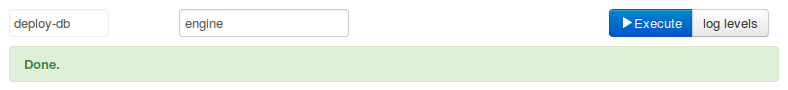
\includegraphics[width=\textwidth]{cmdDone.png}
  \caption{Déploiement réussi de la base de données pour l'infra engine}
\end{figure}

Un message \textbf{Failed!} est accompagné de l'exception Scala émise par
l'application.

\begin{figure}[H]
  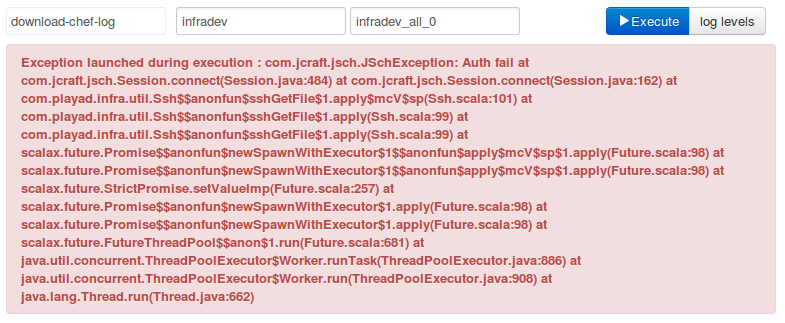
\includegraphics[width=\textwidth]{cmdFailed.png}
  \caption{Échec de la récupération des logs Chef sur le nœud infradev\_all\_0.\\
    L'application ne peut apparemment pas se connecter sur l'instance EC2 de
    ce nœud car l'authentification a échoué}
\end{figure}

\underline{\textit{Bilan}} : Ce message est mis en avant en haut de page,
l'utilisateur ne peut pas le manquer.
Il n'est plus nécessaire de scruter le défilement des logs pour savoir si la
commande est toujours en cours d'exécution. Avec ce message d'alerte qui
s'affiche dynamiquement, on voit tout de suite lorsque la commande s'est
terminée, si elle a réussi ou échoué.

\section{Verrous sur les commandes à effet de bord}

\underline{\textit{La demande}} : interdire l'exécution de deux commandes
identiques en même temps si celles-ci ont des effets de bord.

L'application web côté serveur enregistre les commandes en cours d'exécution.
À chaque nouvelle exécution d'une commande, l'application verrouille toute autre
exécution de la même commande. Lorsque la commande est terminée, qu'elle ait
réussi ou qu'elle ait échoué, l'application enlève le verrou.

Pour cela, l'application maintient un HashSet des commandes en cours d'exécution
qui sont verrouillées. L'ajout ou la suppression du verrou se traduit par un
ajout ou une suppression du nom de la commande dans le HashSet.

Si un utilisateur exécute une commande qui est déjà en cours d'exécution
(i.e. présente dans le HashSet) par un autre utilisateur, l'application renvoie
alors un message d'alerte à l'utilisateur lui indiquant que sa commande est refusée.

\begin{figure}[H]
  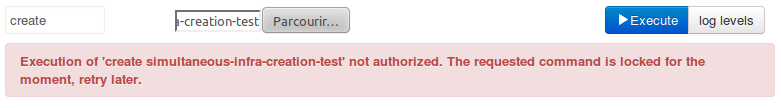
\includegraphics[width=\textwidth]{cmdLocked.png}
  \caption{La commande 'create simultaneous-infra-creation-test' est déjà en
    cours d'exécution.}
\end{figure}

Certaines commandes n'ont pas de verrou car elles n'ont pas d'effet de bord.
Par exemple les commandes status, status-services et show n'ont pas besoin
de verrou car elles ne font que récupérer des informations concernant une infra.

\underline{\textit{Bilan}} : Le verrouillage d'une commande à risque n'est
assuré que si toutes les opérations se font via l'interface web. C'est la webapp
côté serveur qui fait le contrôle. L'outil d'infra en ligne de commande, lui ne
verrouille aucune commande.

\section{Fonctionnalités de la webapp}

\subsection{Complétion automatique des infras}

L'application web fournit une complétion automatique des noms d'infrastructures
pour les champs qui requièrent une infra.

\begin{figure}[H]
  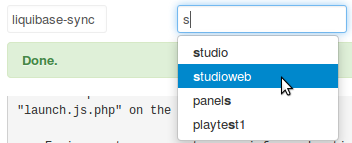
\includegraphics[scale=1]{auto-completion.png}
  \caption{Complétion automatique des noms d'infrastructures disponibles}
\end{figure}

La liste déroulante assiste l'utilisateur lorsqu'il doit indiquer
l'infrastructure sur laquelle s'appliquera sa commande.
Cette fonctionnalité améliore l'expérience utilisateur, l'utilisateur gagne du
temps et évite les erreurs de frappe.

C'est le plugin JavaScript Typeahead de Twitter Bootstrap qui est utilisé pour
avoir ce design sympathique. L'internaute tape quelques lettres de l'item qu'il
recherche et le plugin affiche les items qui contiennent cette séquence de
lettres en facteur.

Une fois le plugin inclus dans le projet, il faut renseigner l'attribut
\textit{data-source} de la balise input avec les différents choix possibles de
la liste.

\lstset{language=XML}
\begin{lstlisting}[caption=utilisation de bootstrap-typeahead]
  <input type="text" data-provide="typeahead" data-items="4" data-source='[]'>
\end{lstlisting}

Comme présenté dans le code html ci-dessus, la liste est vide au début.
Elle contiendra la liste des infras disponibles qui sera générée côté serveur.

Lorsque l'utilisateur se connecte à l'application, la page web lui est envoyée
instantanément. Il peut exécuter la commande qu'il souhaite mais ne
dispose pas encore de la complétion automatique des infrastructures.

Une WebSocket est utilisée pour remplir dynamiquement cette liste.
En asynchrone, la commande \textit{list} est exécutée côté serveur.
Cette commande récupère la liste de toutes les infrastructures disponibles en
requêtant Chef qui dispose de cette information. La commande \textit{list} met
environ 5 secondes à s'exécuter sur l'instance EC2 qui héberge l'application
web.
Une fois la commande \textit{list} terminée, le serveur envoie cette liste des
infrastructures au client via la WebSocket.
Une fonction JavaScript renseigne alors l'attribut data-source avec
la liste des infrastructures reçue.

Le client ne ressent aucune latence de l'application car les briques essentielles
de l'interface web pour exécuter une commande sont instantanément disponibles.
Les fonctionnalités complémentaires comme l'auto-complétion viennent se greffer
dynamiquement à l'interface et n'altèrent pas la navigation de l'utilisateur.

\underline{\textit{Bilan}} : Cette autocomplétion tire pleinement parti du
modèle asynchrone offert par les \textit{WebSocket}. Cette fonctionnalité met
bien en évidence l'intérêt des \textit{WebSocket} pour créer des pages web qui
se mettent à jour dynamiquement en recevant des informations calculées en
asynchrone. Les pages web peuvent devenir de vraies applications temps réel.

\subsection{Défilement automatique des logs de la commande en cours d'exécution}

\begin{figure}[H]
  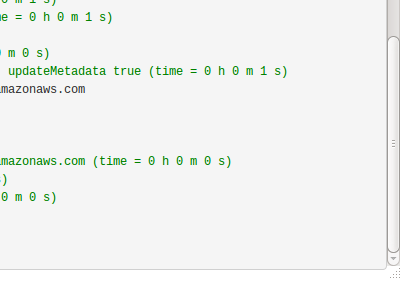
\includegraphics[width=0.50\textwidth]{defilement-automatique-1.png}
  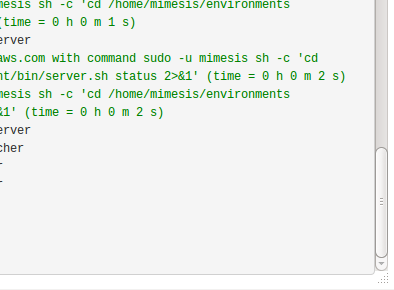
\includegraphics[width=0.50\textwidth]{defilement-automatique-2.png}
  \caption{Défilement automatique des logs - exécution de la commande
    status-services panel\\L'image de droite est prise 4 secondes après celle de gauche}
\end{figure}

Lorsqu'une nouvelle ligne est ajoutée à la suite de l'output du résultat de la
commande, la barre de défilement se met automatiquement en bas.

Si l'utilisateur déplace la barre de défilement, le défilement automatique se
désactive.
Si l'utilisateur replace manuellement la barre de défilement tout en bas,
le défilement automatique est de nouveau actif.

\underline{\textit{Bilan}} : Aucun plugin n'est utilisé ici. Quelques lignes de
JavaScript suffisent pour créer ce système de défilement automatique.

%% \subsection{couleurs des logs}
\subsection{Contrôler les niveaux de log}

Avant d'exécuter une commande, les niveaux de logs peuvent être activés ou
désactivés. Les informations affichées au cours de l'exécution de la commande
sont alors filtrées pour n'afficher que celles correspondant aux niveaux de logs.
Il y a cinq niveaux de logs utilisés dans l'application : 
Trace, Debug, Info, Warn et Error.
Par défaut, tous les niveaux de logs sont activés.

\begin{figure}[H]
  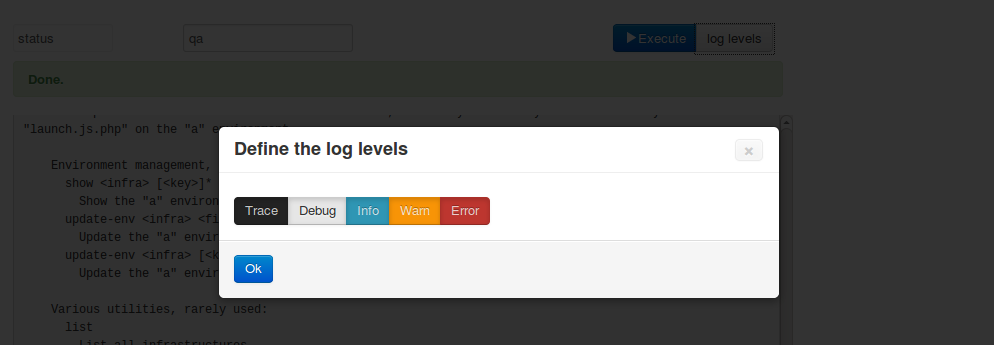
\includegraphics[width=\textwidth]{log-levels.png}
  \caption{Tous les niveaux de logs sont activés}
\end{figure}

\bigskip

La commande \textit{status} fait un appel au logger.debug durant son exécution.
Un utilisateur laissera le niveau Info actif et désactivera Debug
si il souhaite uniquement recevoir le résultat du \textit{status} et ne veut pas
être encombré des tous les logs de Debug.
Du coup, lors de l'exécution de la commande \textit{status qaz}, la ligne
\verb?EXEC: Perform get on data/infrastructures/qaz? ne sera pas affichée car le
niveau Debug a été désactivé par l'utilisateur.

\underline{\textit{Bilan}} : Ce filtrage des niveaux de log est apprécié des
utilisateurs. Il était souvent reproché que la sortie console d'une commande
était beaucoup trop verbeuse. À présent, l'internaute peut régler le niveau de
log à sa convenance.

\subsection{La commande download-chef-log}
La création et la mise à jour d'une infra sont des tâches délicates qui peuvent
souvent échouer.
La cause de cet échec peut varier.
Ça peut venir par exemple de la création de la base de donnée RDS qui ne s'est
pas correctement terminée comme ça peut aussi venir de la limite du nombre de
groupes de sécurité fixée par Amazon qui est atteinte.

Mais la cause la plus fréquente est l'échec de l'exécution du chef-client.
À chaque fois que ce programme plante, un administrateur système doit récupérer le
fichier de logs Chef pour connaître la cause. Il recherche alors sur amazon
l'url de l'instance EC2 qui héberge l'infrastructure car c'est cette instance
qui exécute chef-client et qui possède les logs Chef. Une fois cette url
trouvée, il peut se connecter à l'instance via ssh et récupérer le fichier de
log.

Pour éviter cette tâche fastidieuse aux administrateurs systèmes, la commande
\textit{download-chef-log} a fait son apparition dans l'application web.

Depuis l'interface web, il suffit de renseigner deux champs pour récupérer le
fichier de log. Un premier champ doit contenir le nom de l'infrastructure et un
deuxième doit contenir le nom du nœud sur lequel la commande a échoué.

Contrairement à l'url de l'instance qui n'était pas connu par l'administrateur
système et qu'il devait rechercher sur Amazon, il connaît déjà le nom d'infra et
le nom du nœud.

De plus, pour faciliter son utilisation, les deux champs de cette nouvelle
commande \textit{download-chef-log} possèdent la complétion automatique.

\begin{figure}[H]
  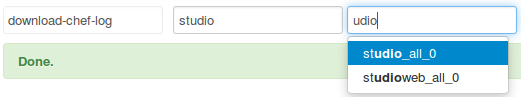
\includegraphics[width=\textwidth]{completion-download-chef-log.png}
  \caption{Complétion automatique disponible aussi pour la liste des nœuds}
\end{figure}

À partir du nom de l'infra et du nœud, le serveur web requête Chef pour
connaître l'url de l'instance EC2 correspondante. En utilisant la commande
\textit{scp}, le serveur copie le fichier de logs Chef distant dans un
dossier local publique.
L'application génère ensuite une URL qui pointe sur le fichier local téléchargé
et envoie cette URL au client.
L'URL est alors affichée sur la page web de l'utilisateur. Il lui suffit de
cliquer dessus pour télécharger le fichier de log qu'il recherchait.


\begin{figure}[H]
  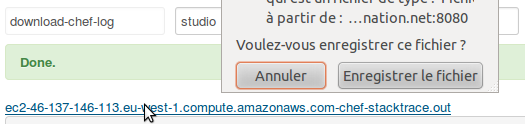
\includegraphics[width=\textwidth]{download-chef-log.png}
  \caption{Lien de téléchargement du fichier de log généré par la commande \textit{download-chef-log}}
\end{figure}

\underline{\textit{Bilan}} : Cette commande est principalement utilisée par les
administrateurs système de la société. Cependant, ils ne peuvent pas se servir
de l'outil en ligne de commande pour l'exécuter car elle n'existe que pour
l'application web.

\clearpage
\section{Évolutions de l'outil d'infra}

\subsection{Création d'infrastructure}

\subsubsection{Des logs plus complets}

Lors de la création d'infra, l'outil appelle le programme \textit{chef-client}
sur chaque instance EC2 de l'infra. 

\underline{\textit{L'objectif}} : Récupérer les logs de la commande chef-client
en cours d'exécution sur l'instance EC2 distante pour pouvoir les afficher à
l'utilisateur.

Le programme \textit{chef-client} initialise toutes les données Chef.
C'est aussi l'étape qui prend le plus de temps à s'exécuter lors d'une création
d'infrastructure.

Une session ssh est ouverte avec la lib Java jsch sur l'instance EC2 qui va
exécuter le chef-client. On ouvre un channel de type \textit{exec} sur lequel on
définit notre logger et la commande à exécuter (i.e. \textit{chef-client}).

\underline{\textit{Bilan}} : Un point négatif est que les logs du
\textit{chef-client} sont assez volumineux. Le client de l'outil d'infra 
peut donc être submergé par toutes ces informations. À trop voir de détails, on
finit par les ignorer. Mais tout de même, lorsqu'une erreur se produit,
l'utilisateur dispose maintenant de toutes les informations d'exécution puisque
tous les logs de n'importe quel programme externe appelé par l'outil d'infra
sont affichés.

%% - afficher les logs du chef-client dans la sortie web lors d'une création
%% d'infra.

\subsubsection{Un nouveau groupe de sécurité de RDS pour chaque nouvelle infra}

L'outil d'infra utilisait le groupe de sécurité RDS par défaut pour les bases de
données associées à une instance. Un nombre limité d'instances EC2 peut être
associé à un groupe de sécurité RDS et cette limite éteinte.

\underline{\textit{L'objectif}} : Créer un nouveau groupe de sécurité RDS pour chaque
\textit{create} d'une nouvelle infra. 

La priorité est haute car la création d'une nouvelle infrastructure ne
fonctionne plus. Le patch est rapidement créé et une nouvelle version de l'outil
d'infra est publiée pour que tout le monde puisse de nouveau créer une
infrastructure avec l'outil.

\underline{\textit{Bilan}} : L'ajout du code pour ce patch dans le temps imparti
montre que je maîtrise à présent le code de l'outil d'infra.

%% - J'ai écris le code qui créé un nouveau db security group rds à chaque fois
%% qu'une nouvelle infra est créée.
%% Ça permettra d'éviter la limite qu'on atteint rapidement lorsqu'on utilise le
%% security group 'default'.


\subsubsection{Des vérifications supplémentaires au début de l'exécution}

\underline{\textit{L'objectif}} : Rajouter des vérifications au début de
l'exécution de la commande \textit{create} pour éviter qu'elle n'échoue plus
tard dans l'exécution.

\begin{itemize}
\item[\textbullet] Les instances de type \textit{t1.micro} n'ont pas assez de
  mémoire pour héberger une infra MambaNation.
  À présent, l'outil d'infra peut détecter et interdire la création d'une
  infrastructure sur ce type d'instance Amazon dès le début de l'exécution de la
  commande \textit{create}.
\item[\textbullet] Une autre vérification empêche la création d'infrastructure
  dont le nom contient une majuscule car les noms avec majuscules ne sont pas
  autorisés pour les Bucket S3.
\end{itemize}


\underline{\textit{Bilan}} :  Il ne sert à rien d'exécuter une création d'une
infrastructure s' il est possible de détecter à l'avance qu'elle va échouer.  
Ces vérifications permettent de détecter une erreur plus tôt et d'afficher des
messages d'erreurs court et explicites.

%% - J'ai rajouté un check dans l'outil d'infra pour interdire le create sur une
%%  parce-que la création d'infra sur une t1.micro ne fonctionne pas, pas
%% assez de mémoire disponible sur les micros probablement.
%% J'ai rajouté un autre check qui vérifie que le nom de l'infra ne contient pas de
%% majuscule.


%% - J'ai fait en sorte de pouvoir créer des infras même sans service mongodb.


\subsection{Optimisations en temps d'exécution}

La commande \textit{registerDns} enregistre un nouveau nom DNS sur AWS Route53
pour chaque nœud de l'infrastructure précisée en entrée de la
commande. \textit{registerDns} met ensuite à jour Chef pour indiquer les
nouveaux DNS assignés.

\subsubsection{Exécution parallèle}

Les enregistrements de ces noms de domaine sont indépendants les uns des autres.
Cette commande a donc été modifié pour que \underline{chaque enregistrement DNS
  s'exécute en parallèle des autres}.

\subsubsection{La manière d'utiliser cette méthode ne change pas}

La méthode registerDns correspondant à la commande du même nom possède un point
de jointure à la fin de son code. Bien que tous les enregistrements soient
effectués en parallèle, la méthode s'assure que tous les enregistrements DNS
sont bien terminés au niveau du point de jointure. 
Ainsi l'utilisateur de la méthode registerDns peut chaîner un appel à une autre
méthode avec la certitude que cette deuxième méthode ne sera appelée uniquement
si tous les enregistrements DNS se sont bien exécutés.

La manière d'utiliser cette méthode ne change pas pour l'utilisateur et le
nouveau code source de la méthode reste compatible avec le reste du code
existant de l'outil.

\subsubsection{Implémentation}

Toutes les classes de l'outil d'infra utilisent la bibliothèque des
\textit{Promises} de MimesisRepublic.
Les \textit{Promises} sont une bonne solution pour exécuter plusieurs opérations
en parallèle d'une manière efficace et non bloquante.

La type de retour de la méthode registerDns est
\textit{Promise[StartedInfrastructure]}.

L'instance de StartedInfrastructure contenue dans la Promise retournée
représente la nouvelle infrastructure dont les DNS ont bien été enregistrés.
Cette Promise contient une StartedInfrastructure qui n'existe pas encore mais
qui pourra être récupérée plus tard.
Voici le code source de la méthode registerDns avec des commentaires rajoutés en
français pour détailler ce qu'elle fait.
\lstset{language=Scala}
\begin{lstlisting}
  class StartedInfrastructure {
    ...

    def registerDns() : Promise[StartedInfrastructure] = 
    logger.logPromOp("Register DNS for infrastructure percentageSigns".format(infraName)) {

      // la méthode join est notre point de jointure.
      def registerAllDns = Promise.join(startedNodes.map { node => node.registerDns(infraName, topDomain) }.toList)

      // méthode qui met a jour l'attribut db_servers_list dans Chef.
      def updateDbServerList() : Unit =
      getNodeWithRole("mongodb_server").headOption.map { 
        node =>
        val newBrmStructure = dbServersList("brm").updated("host", node.privateIp)
        .updated("server_id", node.nodeName)

        val newDbServersList = dbServersList.updated("brm", newBrmStructure)
        structure = structure.updated("db_servers_list", newDbServersList)
        val json = Json.build(structure)
        chef.saveDataBagItem(rootDataBagPath, infraName, json)
      }

      // chaînage des différentes tâches avec la méthode map de la classe Promise :
      // tous les enregistrements DNS sont effectués (registerAllDns) puis les
      // données sont mises à jour dans Chef (updateDbServerList) puis l'instance 
      // de StartedInfrastructure est retournée (this).
      registerAllDns.map { xs => updateDbServerList(); xs }.map(xs => this)
    }
  }
\end{lstlisting}

\underline{\textit{Bilan}} : La méthode registerDns est exécutée par plusieurs commandes
dont \textit{create}, \textit{start}, \textit{restart-services} et
\textit{registerDns}. L'optimisation de cette méthode permet par exemple de
gagner environ 10 secondes lors de la création d'une infra avec quatre nœuds.

\subsection{Documentation dans le wiki}

Certaines commandes de l'outil d'infra échouent plus souvent que
d'autres car elles effectuent des opérations délicates tels que le démarrage
d'instance EC2 et l'écriture en base de données. Les commandes de création et de
destruction d'infrastructure, \textit{create} et \textit{destroy}, en font
partie.

Lorsqu'une commande échoue, les logs affichés à l'utilisateur de l'outil d'infra
(en ligne de commande ou web) décrivent son déroulement pas à pas. Mais parfois
les logs ne suffisent pas et sans une bonne connaissance de l'ensemble des
étapes exécutées par ces lourdes commandes, il est très dur de découvrir la
cause de l'échec.

\underline{\textit{La demande :}} documenter le déroulement des commandes \textit{create},
\textit{destroy}, \textit{start} et \textit{stop}.

Toutes les étapes de ces quatre commandes ont donc été documentées dans le wiki
de Mimesis. Cette page de documentation permet de savoir si l'enregistrement des
DNS s'effectue avant ou après l'initialisation de la base de données RDS ou
encore de savoir à quel moment la liste des services est ajoutée dans Chef par
exemple.
L'utilisateur a ainsi une vision plus claire du déroulement de l'exécution de
l'outil d'infra.
Un administrateur système peut se servir de cette documentation pour repérer
l'opération qui a échoué et la réparer manuellement.

\underline{\textit{Bilan}} : La documentation est nécessaire pour garder une certaine
maîtrise sur le travail effectué. Une fois écrite, la documentation offre aussi
une certaine autonomie aux employés. \\
Travaillant sur l'outil d'infrastructure tous les jours, j'ai moi même découvert
des subtilités dans le déroulement de la commande \textit{create} que je ne
connaissais pas. Cette page de documentation permet à tout le monde d'y voir
un peu plus clair sur l'exécution de l'outil d'infra et sert de premier support
lorsqu'une commande échoue.

\clearpage
\section{Plugin SBT}

Afin de faciliter le déploiement d'un service, Mimesis Republic a mis en place
un modèle de déploiement uniforme sur l'ensemble des infrastructures pour tous
les composants applicatifs.

Tout projet packagé dans une archive zip doit respecter une arborescence bien
définie et l'application web Play! n'y échappe pas.

Un fois dézippé, le projet doit avoir la structure suivante :
\begin{itemize}
\item[\textbullet] conf    (contient les fichiers de configurations)
\item[\textbullet] app     (contient les fichiers binaires)
\item[\textbullet] scripts (contient les scripts)
\end{itemize}

Le dossier \textit{scripts} doit contenir un fichier service.sh .
Ce script permet de démarrer, arrêter, redémarrer ou récupérer l'état de
l'application en question.
Son utilisation est simple :
\begin{lstlisting}
  Usage: service.sh { start | stop | restart | status }  
\end{lstlisting}

Les équipes de la société ont créé plusieurs plugins SBT pour automatiser le
packaging de tout type d'application utilisée.
Ainsi, dans n'importe quel sous-projet de la société (projet PHP, Rails ou
autres), pour créer un zip de l'application courante qui respecte la
structure imposée, il suffit de :
\begin{itemize}
\item ouvrir un terminal
\item invoquer l'interpréteur de commandes \textit{sbt}
\item taper la commande \verb?playad-bundle-generate(for standalone)? \\
\end{itemize}

Jusqu'à présent, Mimesis Republic n'avait pas de projet Play! en développement.
Il n'y avait donc pas de plugin SBT existant pour Play!. 
Le plugin SBT PlayadPlayPlugin a donc été créé pour offrir ce packaging 
automatique.
Désormais, la commande \verb?playad-bundle-generate(for standalone)? fonctionne
aussi pour l'application web \textit{infra-admin-web}.
Une fois l'archive dézippée, le dossier \textit{infra-admin-web} contient bien
les dossiers conf, app et scripts avec le script service.sh pour piloter le
serveur web de l'application.

\bigskip
\underline{\textit{Bilan}} : Le modèle de déploiement uniforme est une très
bonne idée. Le démarrage ou l'arrêt d'une application quelconque peut alors être
 automatisé par un outil externe. 
À présent, pour tout projet Play! à venir, il suffira d'utiliser le plugin
\textit{PlayadPlayPlugin} pour pouvoir accéder à la commande qui package
l'application.
Ça n'a pas été simple de coder ce plugin \textit{PlayadPlayPlugin} car SBT nous
force à configurer des composants immuables au travers de Monads. C'est un style
de programmation très proche des langages fonctionnels et très éloigné des
langages impératifs auxquels j'étais habitué. Malgré son nom (Simple Build
Tool), SBT n'est pas n'est pas si simple après tout.



      
\chapter{Bilan du stage}
En prenant du recul sur mon travail, je tire les enseignements suivants :
\begin{itemize}
  \item[\textbullet] déployer une version stable de l'application le plus
    régulièrement possible permet d'avoir plus de retours de la part des
    utilisateurs.

  \item[\textbullet] proposer aux clients de l'application de donner leur avis et leur
    suggestions. Il ne doit y avoir aucune retenue pour faire une proposition
    de fonctionnalité. Même si une fonctionnalité ne sera pas implémentée car le
    coût temps/intérêt est trop fort ou qu'il y a d'autres tâches plus
    prioritaires, il est toujours intéressant d'en discuter.

    Exemple de proposition non implémentée : avoir un système d'authentification
    connecté à Active Directory pour accéder à la webapp. Il aurait ainsi été
    possible de savoir qui exécute une commande et autoriser l'accès depuis
    internet via authentification. La webapp est aujourd'hui accessible
    uniquement en intranet.
    Le trafic entrant est filtré pour se connecter à la webapp. Seuls les postes
    de travail de l'entreprise faisant partie d'une liste spécifique d'IP y ont accès.
    Ce système d'authentification n'a pas été implémenté car d'autres tâches
    étaient plus prioritaires.

  \item[\textbullet] avant d'entreprendre l'implémentation d'une idée personnelle, il est
    préférable de demander aux équipiers ce qu'ils en pensent. Tout le monde
    n'est pas forcément d'accord sur l'intérêt qu'elle peut avoir.
\end{itemize}
C'est donc ma communication que je devrais principalement améliorer.

Faire son stage dans une start-up requiert d'avoir une bonne autonomie.
Les employés ont déjà beaucoup de travail et problèmes qu'ils doivent régler,
aider un stagiaire n'est pas la plus haute priorité. Avec les nombreux projets
effectués durant mon parcours, l'université m'a appris à être autonome et
trouver des solutions. Si tout de même un problème persistait, je pouvais
demander de l'aide à la personne la plus informée qui n'hésitait pas apporter
son aide.

À propos de façon de travailler, c'est la première fois que j'ai fait du
\textit{pair programming} en entreprise.
Cette méthode de travail consiste à programmer à deux devant le même écran,
l'un écrit le code tandis que l'autre passe en revue chaque ligne de code et
fait des suggestions. Cette technique de développement est très utile lorsqu'il
s'agit de transmettre la connaissance d'une base de code à l'autre.

Ce stage m'a aussi donné l'occasion de travailler avec des informaticiens
passionnés et talentueux qui n'hésitent pas à partager leurs connaissances.
C'est un environnement dynamique dans lequel il faut beaucoup travailler mais
qui permet de progresser rapidement pour devenir meilleur développeur.

Tout n'est pas parfait pour autant chez Mimesis Republic.
Le jeu n'est pas encore très répandu. Il est plus stimulant de travailler
sur un projet populaire, connu de tous. Programmer un mini-jeu qui sera
 utilisé par des centaines de milliers de personnes est valorisant pour le
 développeur.

À certains moments, on peut sentir la pression des dirigeants lorsque les
objectifs en terme de nombre de visiteurs n'ont pas été atteints.
Ceci peut venir d'un ordre conceptuel, le jeu ne plaît pas assez.
Ou bien d'un ordre technique, il n'est plus possible de rentrer dans la 3D par
exemple.
Lorsqu'un problème technique grave est rencontré, il doit être réparé dans
rapidement car une heure d'inaccessibilité de la 3D peut faire perdre de
nombreux joueurs qui ne reviendront plus.
Ce sont donc de lourdes responsabilités qui sont confiées aux différentes
équipes qui sont parfois contraintes de rester tard pour corriger un problème
urgent. Ceci est juste une observation, en tant que stagiaire, de tels
responsabilités ne m'ont pas été attribuées.
Il y a beaucoup de travail et beaucoup d'attentes.


      \chapter{Conclusion}

Après les deux premiers mois de stage, l'application web est rendu disponible.
Les premiers retours sont positifs. De nombreuses idées d'améliorations font
aussi surface de la part des nouveaux utilisateurs.
Ces améliorations ont été implémentées au cours du stage.

L'outil web est maintenant utilisé quotidiennement par les différentes équipes
de la société. C'est aujourd'hui l'outil le plus utilisé pour gérer son
infrastructure.

En dehors de l'outil web, j'ai aussi contribué activement à l'évolution de l'outil
d'infra en ligne de commande.

Ce stage fut aussi très enrichissant au niveau technique.\\
J'ai appris à utiliser de nombreux outils évolués (SBT, AWS, Mercurial)
et j'ai également aiguisé mes compétences par la pratique pour ceux que je
connaissais déjà (Scala).\\

Lors de mon stage précédent chez Normation, je développais déjà en Scala et je
souhaitais continuer à l'utiliser. C'est ce langage Scala qui m'a attiré et
c'est pour pouvoir améliorer mes connaissances sur cette technologie que j'ai
voulu travailler chez Mimesis Republic.\\

À l'avenir, je souhaite travailler pour une entreprise semblable à Mimesis
Republic. C'est à dire travailler sur un projet ambitieux, aux cotés de
programmeurs expérimentés et dans une équipe de taille moyenne tout en restant
dans le cadre dynamique qui est celui des start-up.




      \appendix

\chapter{Références}

\section{Typesafe Stack}
\begin{itemize}
\item \href{http://typesafe.com/}{The stack built to scale featuring Scala, Akka and Play (html - typesafe.com)}\\
\verb?http://typesafe.com/?
\end{itemize}

\subsection{Scala}
\begin{itemize}
\item \href{http://www.scala-lang.org/}{The Scala Programming Language (html - scala-lang.org)}\\
\verb?http://www.scala-lang.org/?

\item \href{http://www.artima.com/pins1ed/}{Programming in Scala, First Edition
(html - artima.com)}\\
\verb?http://www.artima.com/pins1ed/?

\item \href{http://docs.scala-lang.org/sips/pending/futures-promises.html}{Futures
and Promises (html - scala-lang.org)}\\
\verb?http://docs.scala-lang.org/sips/pending/futures-promises.html?
\end{itemize}

\subsection{Play framework}
\begin{itemize}
\item \href{http://www.playframework.org/}{The Play framework (html - playframework.org)}\\
\verb?http://www.playframework.org/?
\end{itemize}

\subsection{SBT}
\begin{itemize}
\item \href{https://github.com/harrah/xsbt/wiki/}{xsbt wiki (html - github.com)}\\
\verb?https://github.com/harrah/xsbt/wiki/?
\end{itemize}

\section{Amazon Web Service (AWS)}
\begin{itemize}         
\item \href{http://media.amazonwebservices.com/AWS_Disaster_Recovery.pdf}{Amazon
Web Services - Using AWS for Disaster Recovery (PDF - amazonwebservices.com)}\\
\verb?http://media.amazonwebservices.com/AWS_Disaster_Recovery.pdf?

\item \href{http://media.amazonwebservices.com/AWS_Building_Fault_Tolerant_Applications.pdf}{Amazon
Web Services - Building Fault-Tolerant Applications on AWS (PDF - amazonwebservices.com)}\\
\verb?http://media.amazonwebservices.com/AWS_Building_Fault_Tolerant_Applications.pdf?

\item \href{http://aws.amazon.com/articles/1636185810492479}{Best Practices in
Evaluating Elastic Load Balancing (HTML - http://aws.amazon.com)}\\
\verb?http://aws.amazon.com/articles/1636185810492479?

\item \href{http://d36cz9buwru1tt.cloudfront.net/AWS_Cloud_Best_Practices.pdf}{AWS
- Cloud\_Best\_Practices (PDF - cloudfront.net)}\\
\verb?http://d36cz9buwru1tt.cloudfront.net/AWS_Cloud_Best_Practices.pdf?
\end{itemize}         

\section{Chef}
\begin{itemize}
\item \href{http://www.opscode.com/chef/}{Opscode Chef - Configuration Tool (opscode.com)}\\
\verb?http://www.opscode.com/chef/?
\end{itemize}         
\section{Autres}

\begin{itemize}
\item \href{http://jetty.codehaus.org/jetty/}{The Jetty Web Server (html - codehaus.org)}\\
\verb?http://jetty.codehaus.org/jetty/?

\item \href{http://www.zabbix.com/}{Zabbix- The enterprise class monitoring solution (zabbix.com)}\\
\verb?http://www.zabbix.com/?

\item \href{http://www.oracle.com/technetwork/java/javase/tech/javamanagement-140525.html}{JMX- Java Management Extension (Oracle.com)}\\
\verb?http://www.oracle.com/technetwork/java/javase/tech/javamanagement-140525.html?

\item \href{http://www.rabbitmq.com/}{Rabbit MQ - Messaging Solution (rabbitmq.com)}\\
\verb?http://www.rabbitmq.com/?

\item \href{http://www.mongodb.org/}{Mongo DB - No SQL Database (mongodb.org)}\\
\verb?http://www.mongodb.org/?

\item \href{http://jenkins-ci.org/}{Jenkins- Continuous Integration (jenkins-ci.org)}\\
\verb?http://jenkins-ci.org/?
\end{itemize}


%% \chapter{Description Amazon Instance}

%% References



%% Amazon Instance Description

%% Description of Amazon instance characteristic as of 23th March 2012
%% EC2 Instance Types
%% Standard Instances

%% Instances of this family are well suited for most applications.

%% Small Instance - default*

%% 1.7 GB memory
%% 1 EC2 Compute Unit (1 virtual core with 1 EC2 Compute Unit)
%% 160 GB instance storage
%% 32-bit or 64-bit platform
%% I/O Performance: Moderate
%% API name: m1.small

%% Medium Instance

%% 3.75 GB memory
%% 2 EC2 Compute Unit (1 virtual core with 2 EC2 Compute Unit)
%% 410 GB instance storage
%% 32-bit or 64-bit platform
%% I/O Performance: Moderate
%% API name: m1.medium

%% Large Instance

%% 7.5 GB memory
%% 4 EC2 Compute Units (2 virtual cores with 2 EC2 Compute Units each)
%% 850 GB instance storage
%% 64-bit platform
%% I/O Performance: High
%% API name: m1.large

%% Extra Large Instance

%% 15 GB memory
%% 8 EC2 Compute Units (4 virtual cores with 2 EC2 Compute Units each)
%% 1,690 GB instance storage
%% 64-bit platform
%% I/O Performance: High
%% API name: m1.xlarge
%% High-Memory Instances

%% Instances of this family offer large memory sizes for high throughput applications, including database and memory caching applications.

%% High-Memory Extra Large Instance

%% 17.1 GB of memory
%% 6.5 EC2 Compute Units (2 virtual cores with 3.25 EC2 Compute Units each)
%% 420 GB of instance storage
%% 64-bit platform
%% I/O Performance: Moderate
%% API name: m2.xlarge

%% High-Memory Double Extra Large Instance

%% 34.2 GB of memory
%% 13 EC2 Compute Units (4 virtual cores with 3.25 EC2 Compute Units each)
%% 850 GB of instance storage
%% 64-bit platform
%% I/O Performance: High
%% API name: m2.2xlarge

%% High-Memory Quadruple Extra Large Instance

%% 68.4 GB of memory
%% 26 EC2 Compute Units (8 virtual cores with 3.25 EC2 Compute Units each)
%% 1690 GB of instance storage
%% 64-bit platform
%% I/O Performance: High
%% API name: m2.4xlarge
%% High-CPU Instances

%% Instances of this family have proportionally more CPU resources than memory (RAM) and are well suited for compute-intensive applications.

%% High-CPU Medium Instance

%% 1.7 GB of memory
%% 5 EC2 Compute Units (2 virtual cores with 2.5 EC2 Compute Units each)
%% 350 GB of instance storage
%% 32-bit or 64-bit platform
%% I/O Performance: Moderate
%% API name: c1.medium

%% High-CPU Extra Large Instance

%% 7 GB of memory
%% 20 EC2 Compute Units (8 virtual cores with 2.5 EC2 Compute Units each)
%% 1690 GB of instance storage
%% 64-bit platform
%% I/O Performance: High
%% API name: c1.xlarge
%% RDS Instance Classes

%%     Small DB Instance: 1.7 GB memory, 1 ECU (1 virtual core with 1 ECU), 64-bit platform, Moderate I/O Capacity

%%     Large DB Instance: 7.5 GB memory, 4 ECUs (2 virtual cores with 2 ECUs each), 64-bit platform, High I/O Capacity

%%     Extra Large DB Instance: 15 GB of memory, 8 ECUs (4 virtual cores with 2 ECUs each), 64-bit platform, High I/O Capacity (MySQL DB Engine Only)

%%     High-Memory Extra Large Instance 17.1 GB memory, 6.5 ECU (2 virtual cores with 3.25 ECUs each), 64-bit platform, High I/O Capacity

%%     High-Memory Double Extra Large DB Instance: 34 GB of memory, 13 ECUs (4 virtual cores with 3,25 ECUs each), 64-bit platform, High I/O Capacity

%%     High-Memory Quadruple Extra Large DB Instance: 68 GB of memory, 26 ECUs (8 virtual cores with 3.25 ECUs each), 64-bit platform, High I/O Capacity 


    \end{onehalfspace}             % Pour finir l'interligne de 1,5

    \end{document}
    %%%%%%%%%%%%%%%%%%%%%%%%%%%%%%%%%%%%%%%%%%%%%%%%%%%%%%%%%%%%%%%%%%%%%%%%%%%%%%%%


